\documentclass[10pt, a4paper]{article}

\usepackage[utf8]{inputenc}
\usepackage[english, spanish]{babel}
\usepackage[left=25mm, right=25mm, top=35mm, bottom=30mm, headheight=35mm]{geometry}
\usepackage{graphicx}
\usepackage{float}
\usepackage{xcolor}
\usepackage{fancyhdr}
\usepackage{hyperref}
\usepackage{setspace}
\usepackage{indentfirst}

% Syntax customization
\usepackage{minted}
\usemintedstyle{nord}
\setminted{
  breaklines,
  linenos,
  frame=lines,
  fontsize=\footnotesize
}

% Define background color
\definecolor{background}{HTML}{2E3440}

% Variables
\newcommand{\university}{Universidad Nacional de San Agustín de Arequipa}
\newcommand{\faculty}{Facultad de Ingeniería de Producción y Servicios}
\newcommand{\program}{Escuela Profesional de Ingeniería de Sistemas}
\newcommand{\semester}{2024 - A}
\newcommand{\course}{img/web_programming.png}
\newcommand{\topic}{img/ajax.png}
\newcommand{\professor}{Carlo Jose Luis Corrales Delgado}
\newcommand{\students}{Mamani Anahua, Victor Narciso \\ Mamani Huarsaya, Jorge Luis \\  Quispe Marca Edysson Darwin \\Velarde Saldaña Jhossep Fabritzio \\ Zuñiga Villacorta Peter Sebastian} 
\newcommand{\githubOne}{https://github.com/jorghee/tareaAjax}
\newcommand{\githubTwo}{https://github.com/jorghee/ajax-markdown}
\newcommand{\mydate}{18 de mayo, 2024}

% Just parts and chapters numbered
\setcounter{secnumdepth}{0}

% Head and foot customization
\pagestyle{fancy}
\lhead{\raisebox{-0.2\height}{
\includegraphics[width=4cm]{img/logo_unsa.png}}}
\chead{\fontsize{8}{8}\selectfont \university \\ \faculty \\ \textbf{\program}}
\rhead{\raisebox{-0.2\height}{
\includegraphics[width=3.5cm]{img/logo_episunsa.png}}}
\lfoot{Estudiantes \student}
\cfoot{}
\rfoot{Pág. \thepage}

\begin{document}



\begin{titlepage}
	\centering
	\includegraphics[width=14cm]{\course} \par
  \vfill \vfill
	\includegraphics[width=15cm]{\topic}\par
  \vfill \vfill
  {\textbf{Profesor(a):} \par}
	\professor \vfill
  {\textbf{Estudiante:} \par}
	\students \vfill
  {\textbf{Repositorios GitHub:} \par}
  \href{\githubOne}{\githubOne}\\
  \href{\githubTwo}{\githubTwo}\\
  \vfill
  {\large \mydate \par}
\end{titlepage}

\section{Peticiones AJAX a un servidor node.js}

\subsubsection{Creando el directorio que contiene los archivos Markdwon}
Empezamos copiando archivos de ejemplo .md al directorio files\_markdown. Este directorio es el que responde a las peticiones AJAX.

\begin{minted}{zsh}
$ ls --tree
files_markdown
	calculator_with_java.md
	example_readme_github.md
	learning_github.md
	project_ajax_regions.md
	server_with_nodejs.md
\end{minted}

\subsection{Creando el servidor con Express}
En este ocasión vamos a utilizar todos los siguientes paquetes para para poder resolver direcciones a archivos y directorios, escribir y leer archivos en directorios y lo más importante es el uso del paquete \textbf{markdown-it} que se encarga de hacer la conversion de markdown a html.

\begin{minted}[bgcolor=background]{javascript}
const path = require("path");
const fs = require("fs");
const MarkdownIt = require("markdown-it");
const bp = require("body-parser");
const express = require("express");
const app = express();
const md = new MarkdownIt();
const MARKDOWN_DIR = path.resolve(__dirname, "files_markdown");

app.use(bp.json());
app.use(express.static("public"));
\end{minted}

Como se observa, hemos declarado una variable estatica \textbf{MARDOWN\_DIR} que almacena la dirección completa al directorio con el cual vamos a trabajar. Además, se ha configurado para que el servidor sirva archivos estaticos desde el directorio \textbf{public} con el objetivo de organizar mejor nuestro proyecto, ya que aqui se encontraran los archivos html, css y los scripts.
\singlespacing
Ahora podemos servir el archivo \textbf{index.html} para que nuestro proyecto pueda visualizarse.

\begin{minted}[bgcolor=background]{javascript}
/** 
  * Creamos el servidor, request maneja las solicitudes que hacemos y 
  * response es el objeto que maneja las respuestas que envia el servidor.
  */ 
app.get('/', (request, response) => {
  response.sendFile(path.resolve(__dirname, "public/index.html"));
});
\end{minted}

\subsection{Implemetando la función que lista los archivos Markdown}
Lo primero que hacemos es configurar el servidor para que pueda manejar la peticióñ y enviar una respuesta al navegador. Como ahora solo necesitamos leer, vamos a usar el paquete \textbf{fs} de node.js que nos otorga funciones para poder interactuar con el sistema de archivos del sistema operativo donde se encuentra levantado el servidor.\\
\singlespacing
Podemos hacer que el servidor responda en formato \textbf{JSON} como es común hoy en día.

\begin{minted}[bgcolor=background]{javascript}
// Listar archivos Markdown
app.get("/files", (request, response) => {
  fs.readdir(MARKDOWN\_DIR, (error, files) => {
    if (error) {
      console.error("No se pudo leer los archivos:", error);
      return;
    }
    response.json(files);
  });
});
\end{minted}

\subsubsection{Solicitud AJAX}
Ahora que ya hemos configurado el servidor, podemos empezar a contruir nuestra petición AJAX, en este caso usaremos la función \mintinline[style=gruvbox-light]{javascript}{fetch()} para poder manejar las promesas.\\
La solicitud la hacemos a la direccion en la cual ha sido configurada el servidor. Una vez que hecha la peticion, el servidor envía los nombres de los archivos .md y con la funcion \mintinline[style=gruvbox-light]{javascript}{then()} manejamos esta respuesta. 

\begin{minted}[bgcolor=background]{javascript}
function listMarkdownFiles() {
  fetch("/files")
    .then(response => response.json())
    .then(files => {
      let fileList = "";
      files.forEach(file => fileList += `<li>${file}</li>`);
      document.getElementById("files").innerHTML = fileList;
    })
    .catch(error => console.error("Error al listar los archivos:", error));
}

export { listMarkdownFiles };
\end{minted}

Entonces comenzamos iterando por cada valor, que en este caso son los nombres de los archivos, y generamos código html que se encargue de mostrar estos nombres como una lista. La lista que hemos generando con la etiqueta \textbf{li} la ponemos en el elemento de ID files, concluyendo asi la petición ajax.

\begin{figure}[H]
  \centering
  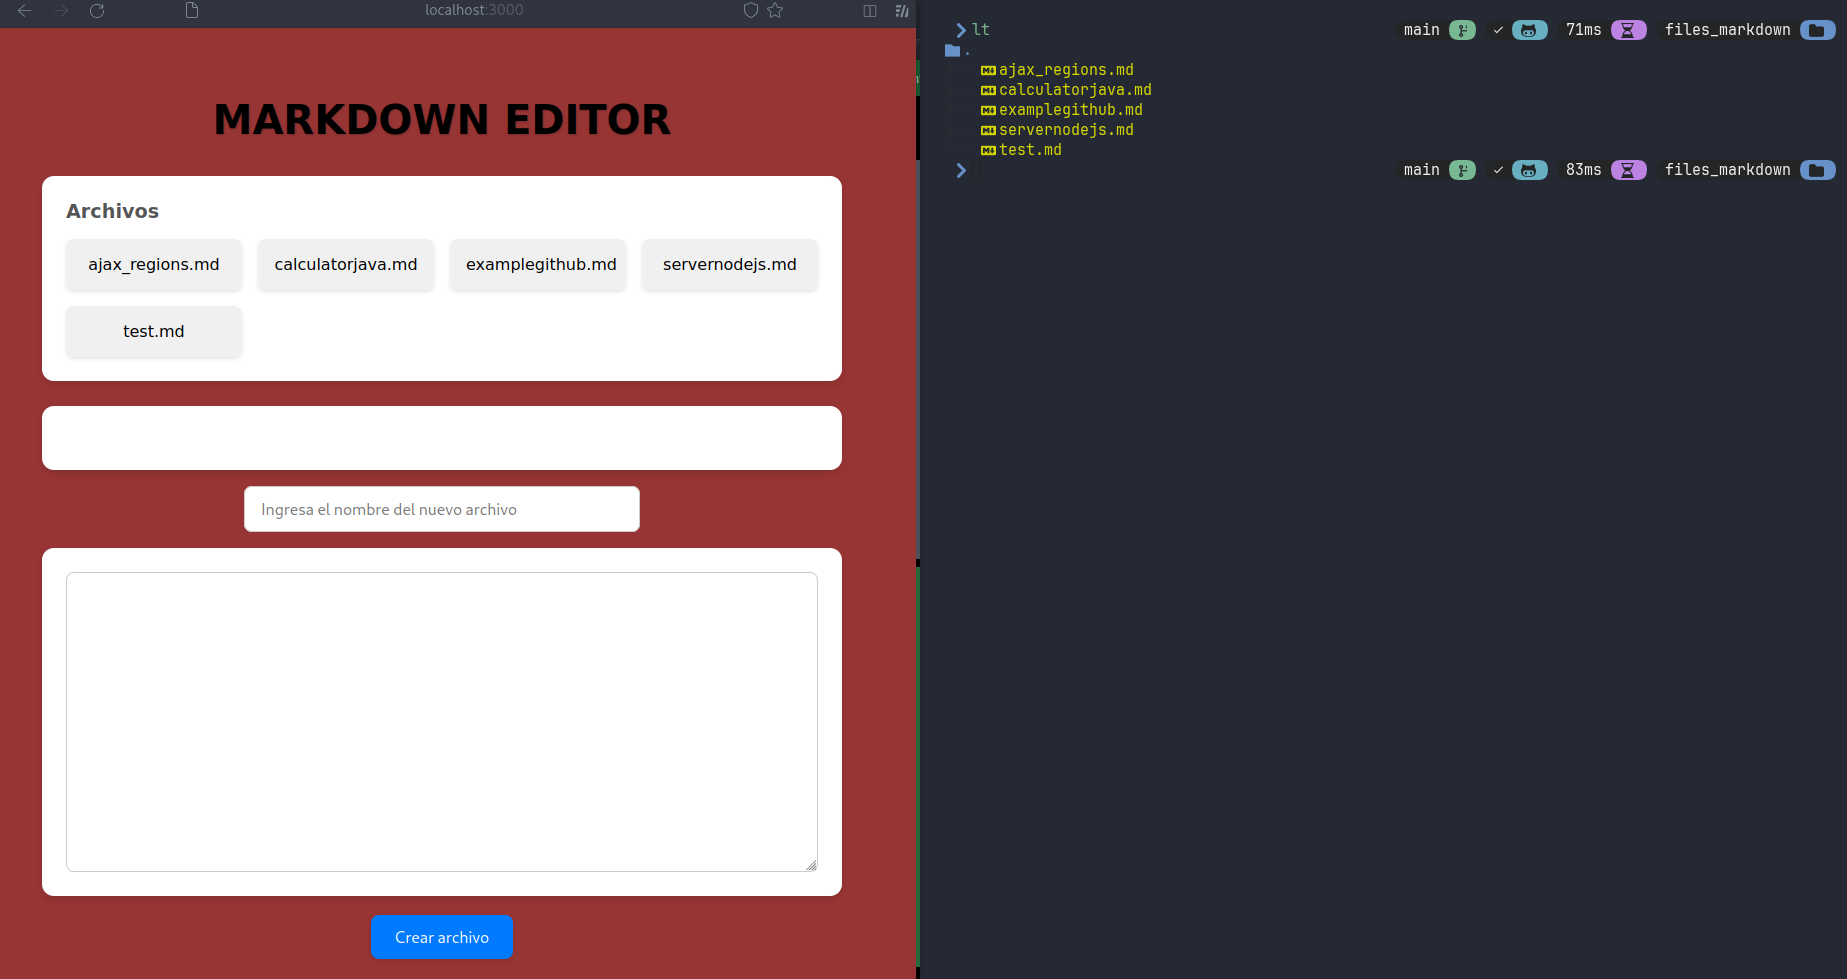
\includegraphics[width=1.0\textwidth]{img/list_markdown.png}
  \caption{Lisrado de los archivos markdown}
\end{figure}

\subsection{Implemetando la función que visualiza un archivo Markdown}
Del mismo modo, nosotros tenemos que implementar la lógica para decirle al servidor cómo debe manejar una solicitud. En este excepcional caso, nos daremos cuenta que necesitamos enviar un identificador que le permita al servidor identificar qué archivo se desea visualizar. Por lo tanto, la configuración debe recibir un parametro.

\begin{minted}[bgcolor=background]{javascript}
app.get('/files/:fileName', (req, res) => {
  const filename = req.params.fileName;
  const filePath = path.resolve(MARKDOWN\_DIR, filename);
  
  fs.readFile(filePath, 'utf8', (err, data) => {
    if (err) {
      return res.status(500).json({ error: "Unable to read file" });
    }
    const htmlContent = md.render(data);
    res.json({html: htmlContent});
  });
});
\end{minted}

Como se observa, el servidor recibe un parametro, dicho parametro es el nombre de archivo que se desea ver. Aqui lo complicado fue pensar cómo recuperar el nombre y enviarle al servidor. Despues veremos que agregando un evento a cada etiqueta \textbf{li} podemos enviar este identificador.
\singlespacing
Con el identificador ya recibido, podemos buscar el archivo en el correspondiente directorio y empezar a leerlo. Sin embargo, lo que hemos leido solo es texto con la extension .md, entonces, aqui usamos el paquete \textbf{markdown-it} que se encarga de hacer la conversion y que pueda ser visualizado por el navegador.

\subsubsection{Realizando la petición AJAX}
Con el servidor configurado, podemos empezar creando la función que se encarga de hacer la petición. La función entonces envia el identificador al servidor y este responde con un texto formateado a html. Basicamente ese el funcionamiento de esta función la cual modifica la etiqueta \textbf{div} de ID content en la cual muestra el texto html.

\begin{minted}[bgcolor=background]{javascript}
export { showMarkdownFile };

function showMarkdownFile(fileName) {
  fetch(`/files/${fileName}`)
    .then(response => {
      if (!response.ok) {
        throw new Error(`HTTP error! status: ${response.status}`);
      }
      return response.json();
    })
    .then(htmlContent => {
      document.getElementById("content").innerHTML = htmlContent.html;
    })
    .catch(error => console.error("Error al mostrar el archivo:", error));
}
  
export { showMarkdownFile };
\end{minted}

\begin{figure}[H]
  \centering
  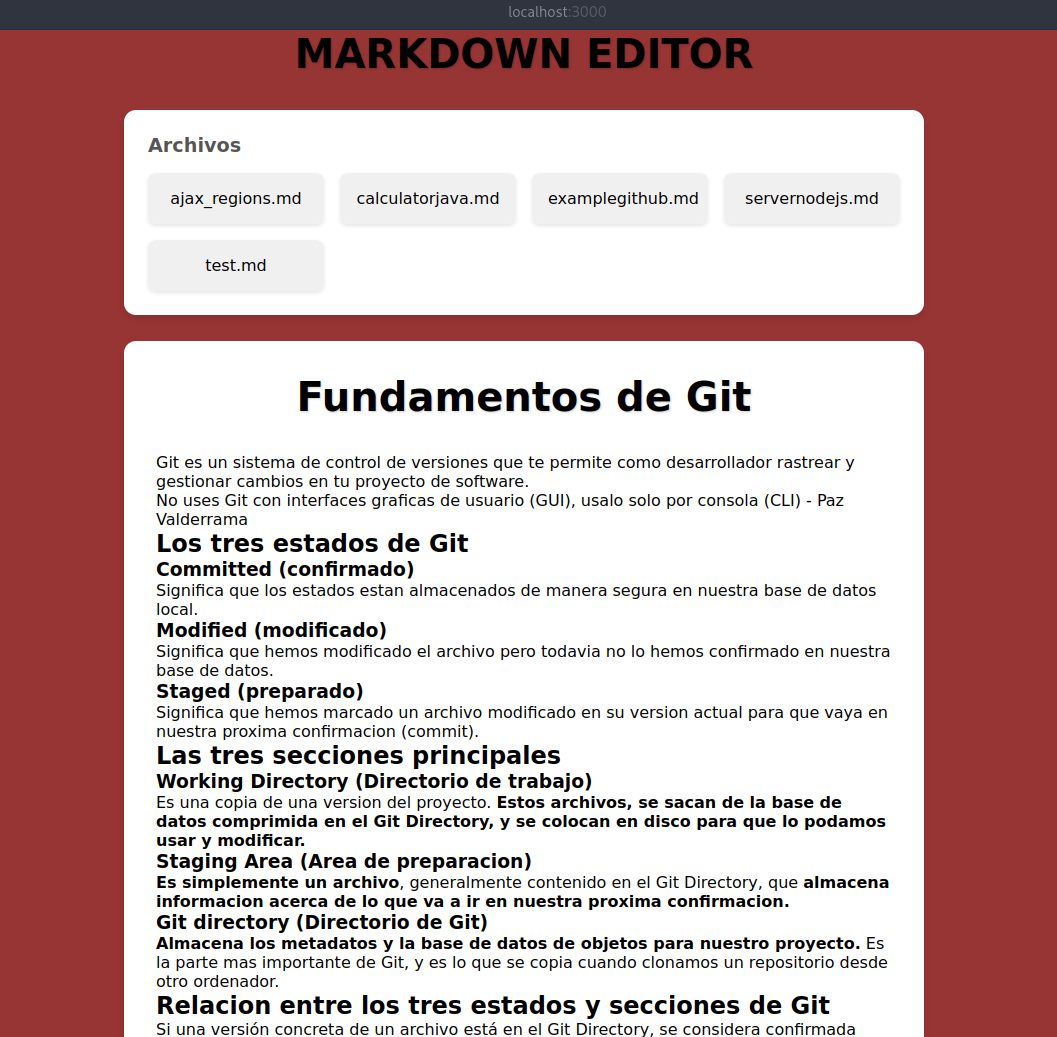
\includegraphics[width=1.0\textwidth]{img/show_markdown.png}
  \caption{Vista de un archivo especifico}
\end{figure}

\subsection{Implemetando la función que crea y almacena un archivo Markdown en el servidor}
Finalmente necesitamos guardar en el servidor los archivos creados en la pagina web. Por lo tanto la funcion especifica del paquete \textbf{fs} que usaremos es \mintinline[style=gruvbox-light]{javascript}{writeFile()}. 
\singlespacing
El servidor necesita recibir el nombre del archivo y el contenido en si del archivo, por ello recuperamos los valores enviamos en el cuerpo de la solicitud y los usamos en el metodo mencionado del paquete \textbf{fs}

\begin{minted}[bgcolor=background]{javascript}
// Crear un archivo
app.post("/files", (request, response) => {
  // Recuperamos los valores
  const { filename, content } = request.body;
  console.log(filename, content);

  const filePath = path.resolve(MARKDOWN_DIR, filename);
  fs.writeFile(filePath, content, error => {
    if (error) {
      console.log(error);
      response.json({ error: "No se pudo crear el archivo" });
    }

    response.json({ message: "Archivo creado existosamente" });
  });
});
\end{minted}

En este caso el servidor no devuelve nada especifico que se deba usar en el cliente, solo necesitamos saber si el almacenamiento del archivo fue existoso.

\subsubsection{Realizando la petición AJAX}
Para poder crear y elegir un nombre para guardar el archivo, hemos creado 2 elementos: \textbf{input} y \textbf{textarea}, entonces necesitamos obtener los valores de estos elementos. Una vez recogidos los valores, lo enviamos en el cuerpo de la solitud ajax. Basicamente en eso consiste la solicitud, finalizando asi las tres funcionalidades de esta pagina web.

\begin{minted}[bgcolor=background]{javascript}
import { listMarkdownFiles } from "./listMarkdown.js";

function createMarkdownFile() {
  const filename = document.getElementById("newFileName").value;
  const content = document.getElementById("newFileContent").value;
  console.log(filename, content);

  // Generamos los parametros de la solicitud
  const request = {
    method: "POST",
    headers: {
      "Content-Type": "application/json",
    },
    
    // Pasamos el objeto con los valores de filename y content
    body: JSON.stringify({ filename, content }),
  };
  
  fetch("/files", request)
    .then(response =>  response.json())
    .then(data => {
      console.log(data.message);
      listMarkdownFiles();
    })
    .catch(error => console.error("Error al crear el archivo", error));
}

export { createMarkdownFile }
\end{minted}

\begin{figure}[H]
  \centering
  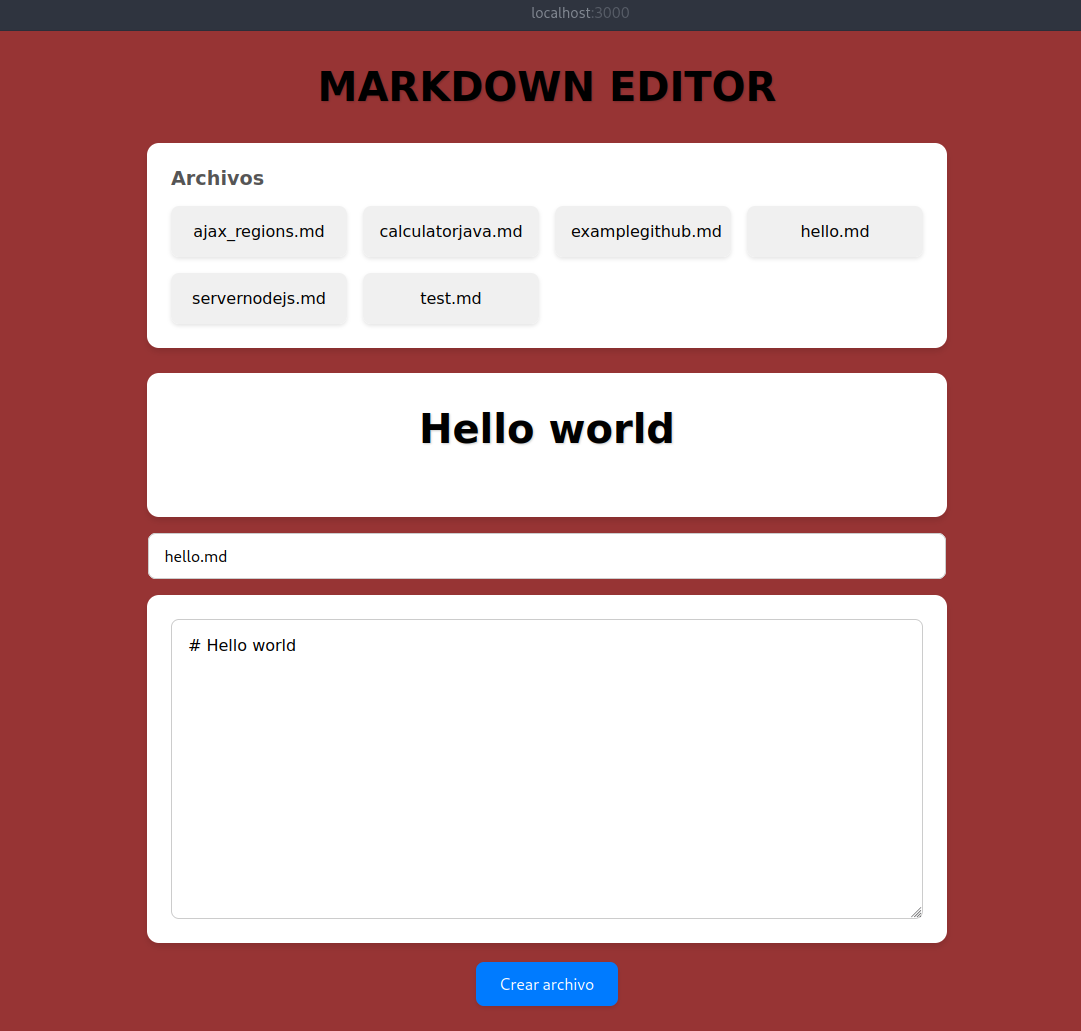
\includegraphics[width=1.0\textwidth]{img/create_markdown.png}
  \caption{Creando archivo y almacenando en el servidor}
\end{figure}

Como se ha observado en todas las funciones de peticion AJAX, al final siempre exportabamos dicha función. Esta idea fue con el objetivo de organizar nuestro proyecto y hacer más manejable en cuanto a los errores.

\begin{minted}[bgcolor=background]{javascript}
import { listMarkdownFiles } from "./listMarkdown.js";
import { showMarkdownFile } from "./showMarkdown.js";
import { createMarkdownFile } from "./createMarkdown.js";

listMarkdownFiles();

document.getElementById('files').addEventListener('click', (event) => {
  if (event.target.tagName === 'LI')
      showMarkdownFile(event.target.textContent);
});

document.getElementById("createFile").addEventListener("click", createMarkdownFile);
\end{minted}


\section{Ejercicios de Ajax en w3schools}

Capturas de pantalla:

\begin{figure}[H]
    \centering
    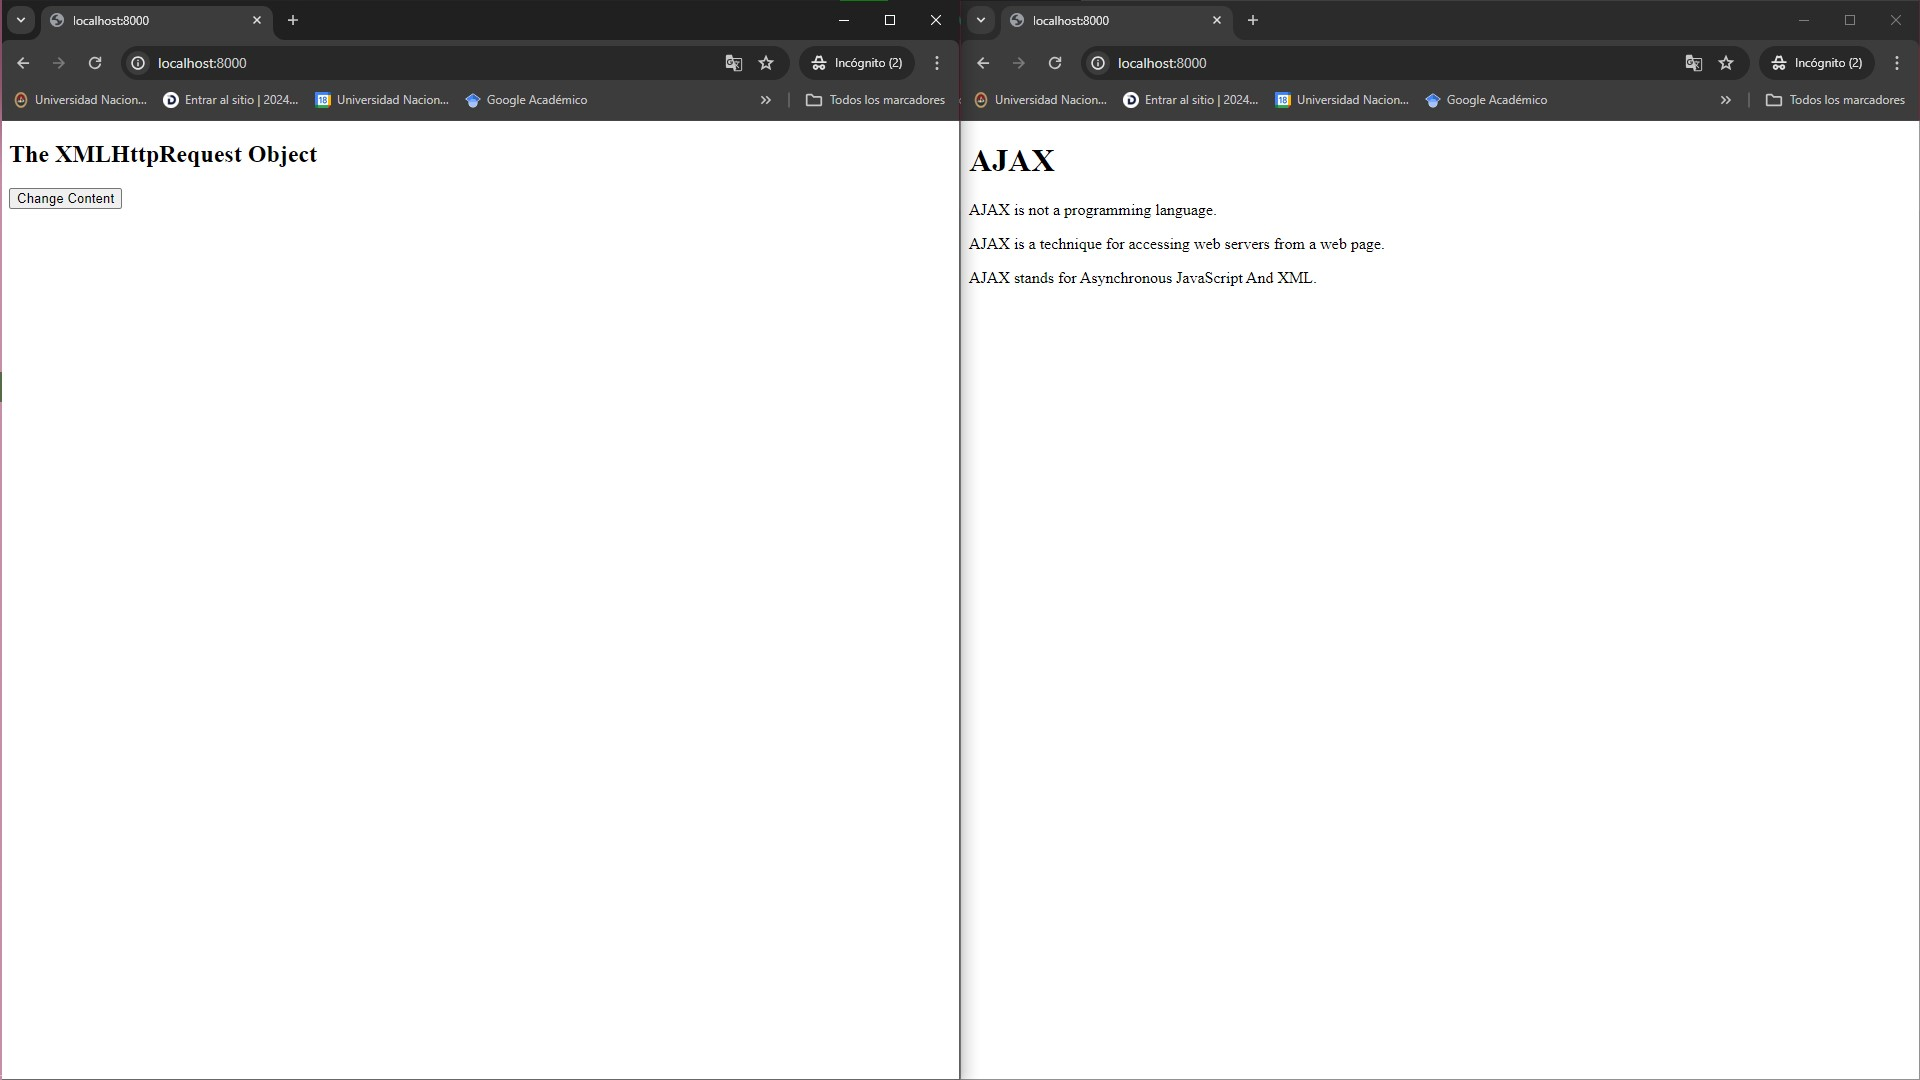
\includegraphics[width=0.7\textwidth]{img/ex1.jpg}
    \caption{Creando un objeto XMLHttpRequest}
    \end{figure}


\begin{figure}[H]
  \centering
  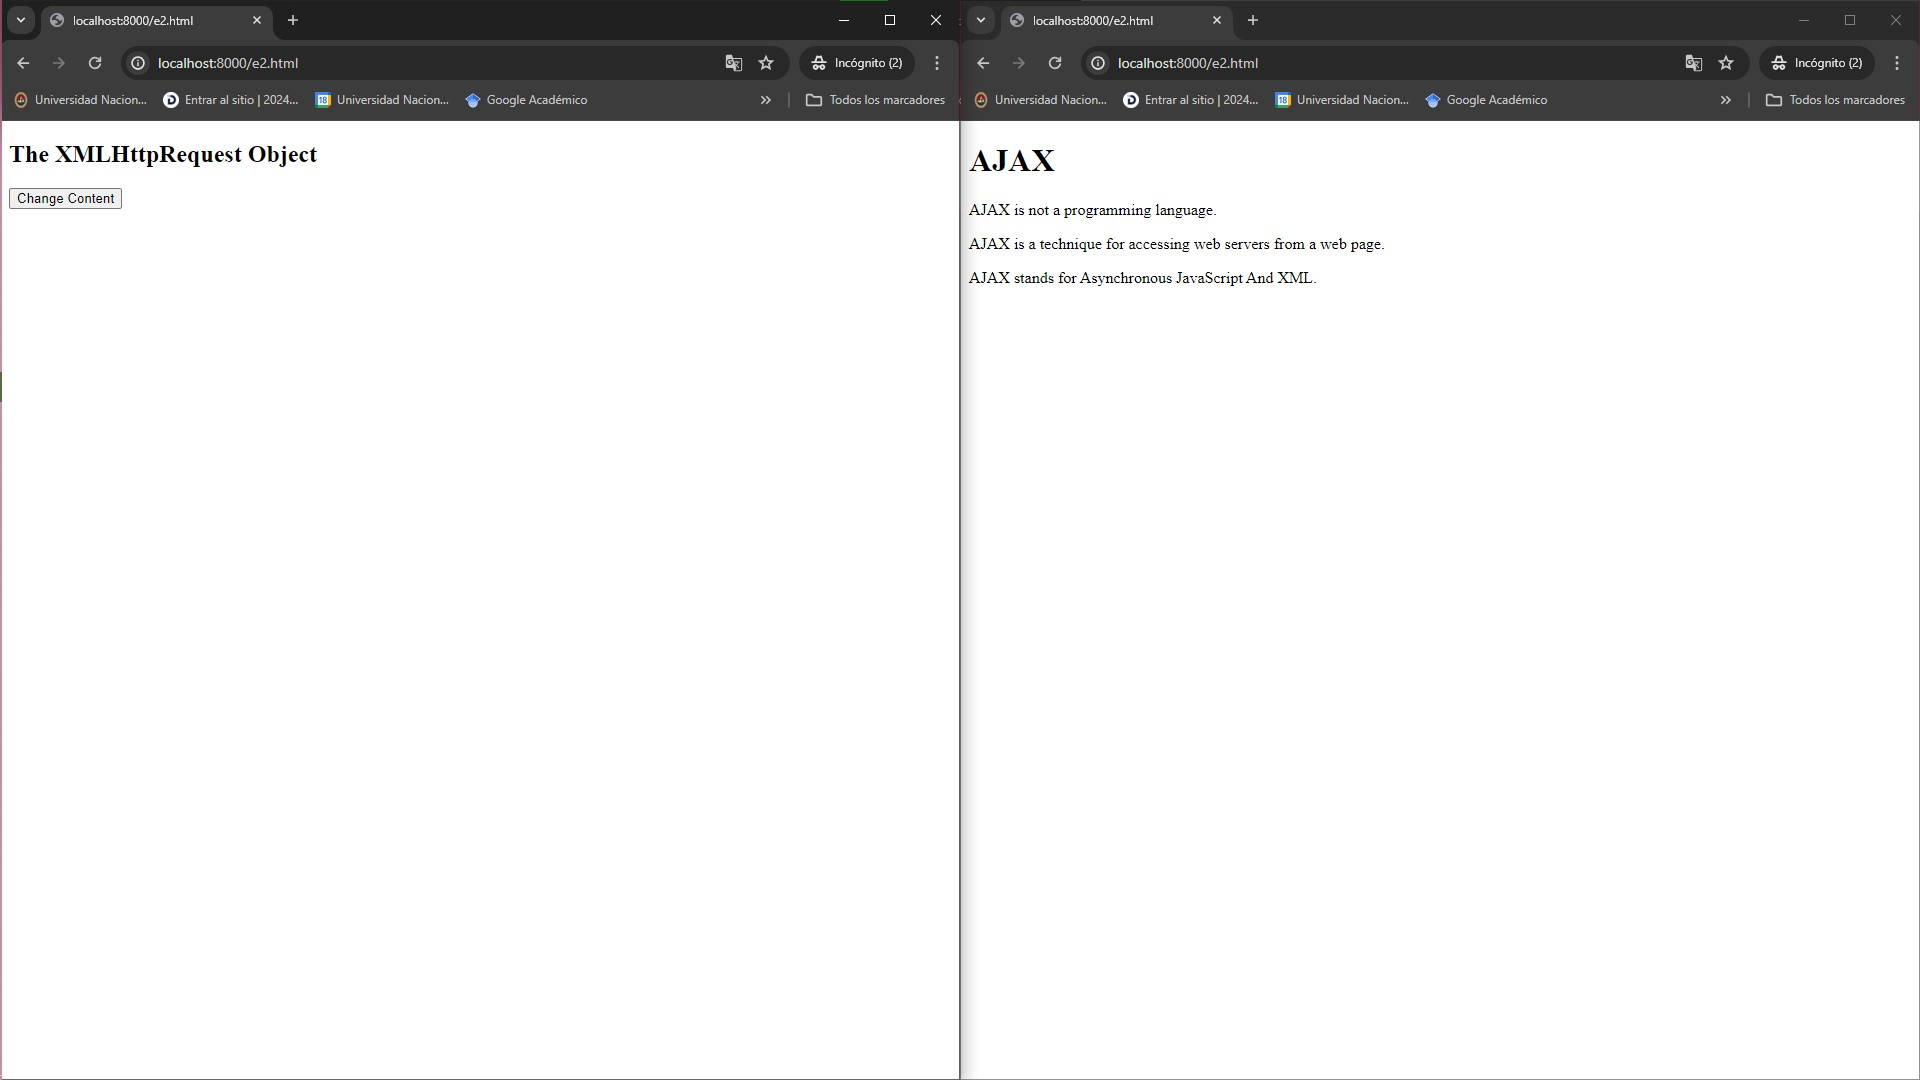
\includegraphics[width=0.7\textwidth]{img/ex2.jpg}
  \caption{Creando otro objeto XMLHttpRequest}
  \end{figure}
\begin{figure}[H]
    \centering
    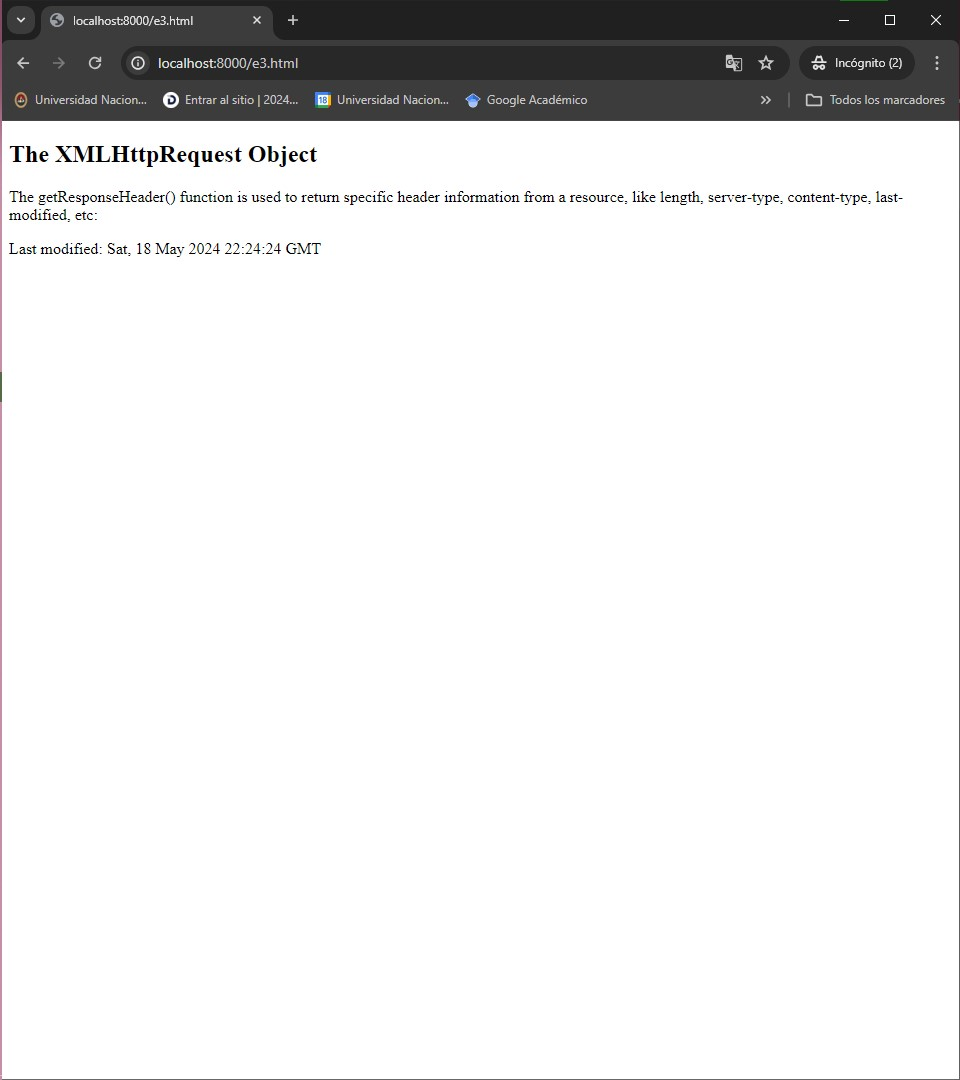
\includegraphics[width=0.5\textwidth]{img/ex3.jpg}
    \caption{Modificando el objeto XMLHttpRequest}
    \end{figure}
\begin{figure}[H]
    \centering
    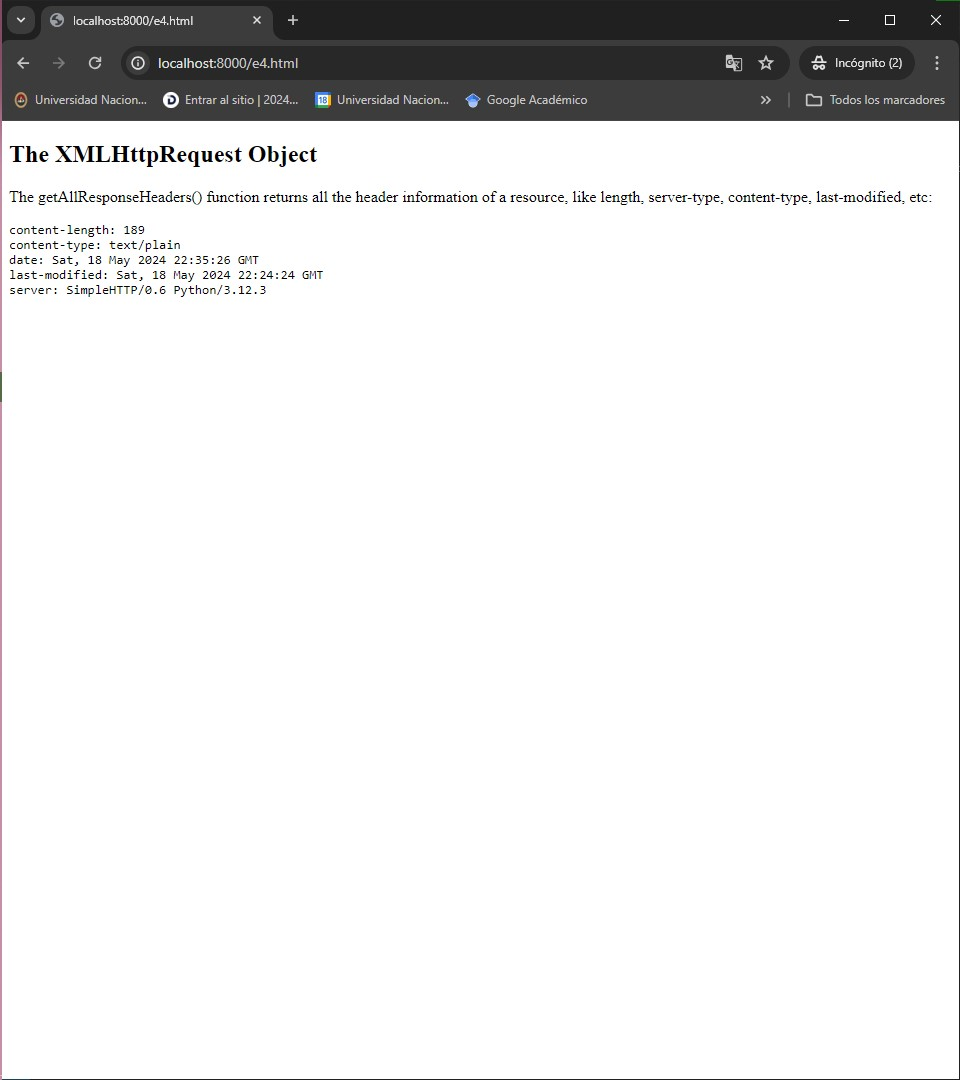
\includegraphics[width=0.5\textwidth]{img/ex4.jpg}
    \caption{Añadiendo contenido al objeto XMLHttpRequest}
    \end{figure}

\begin{figure}[H]
      \centering
      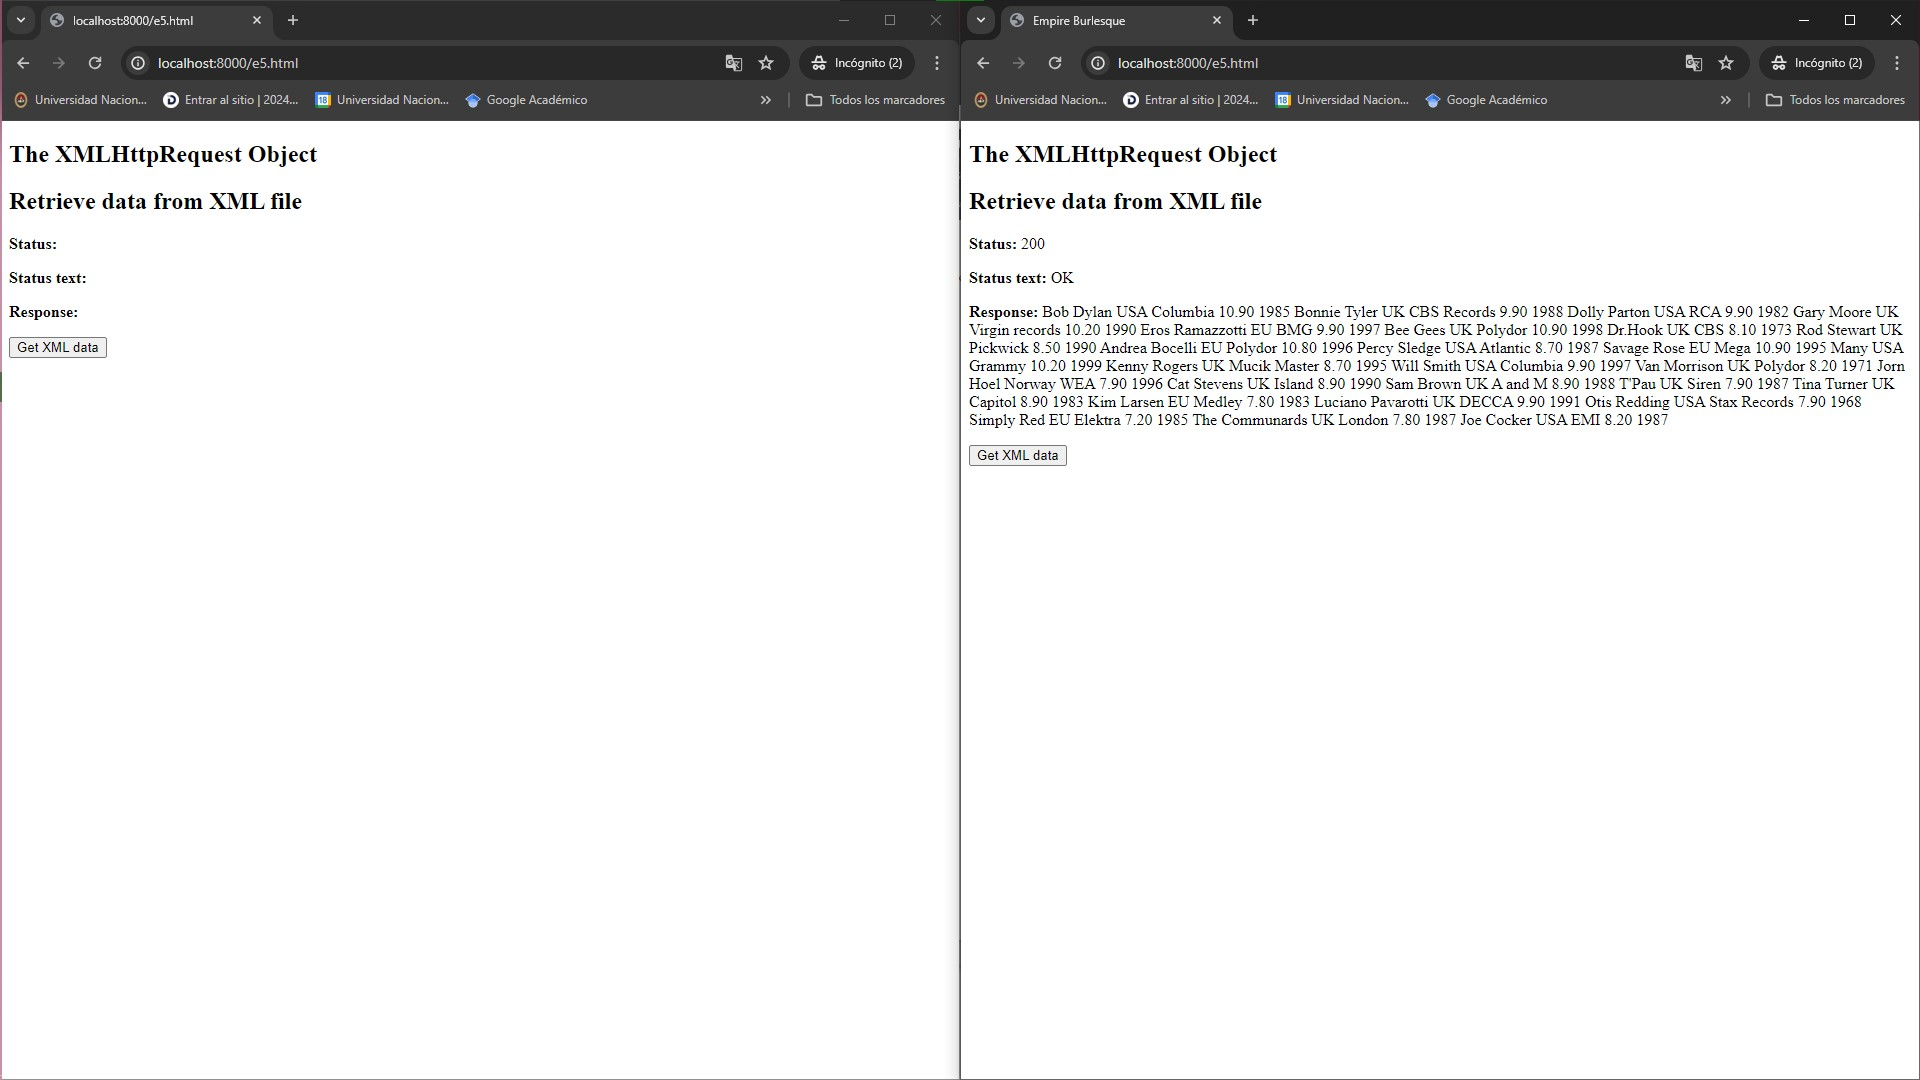
\includegraphics[width=0.7\textwidth]{img/ex5.jpg}
      \caption{Pidiendo un reporte del status del objeto XMLHttpRequest}
      \end{figure}

\begin{figure}[H]
    \centering
    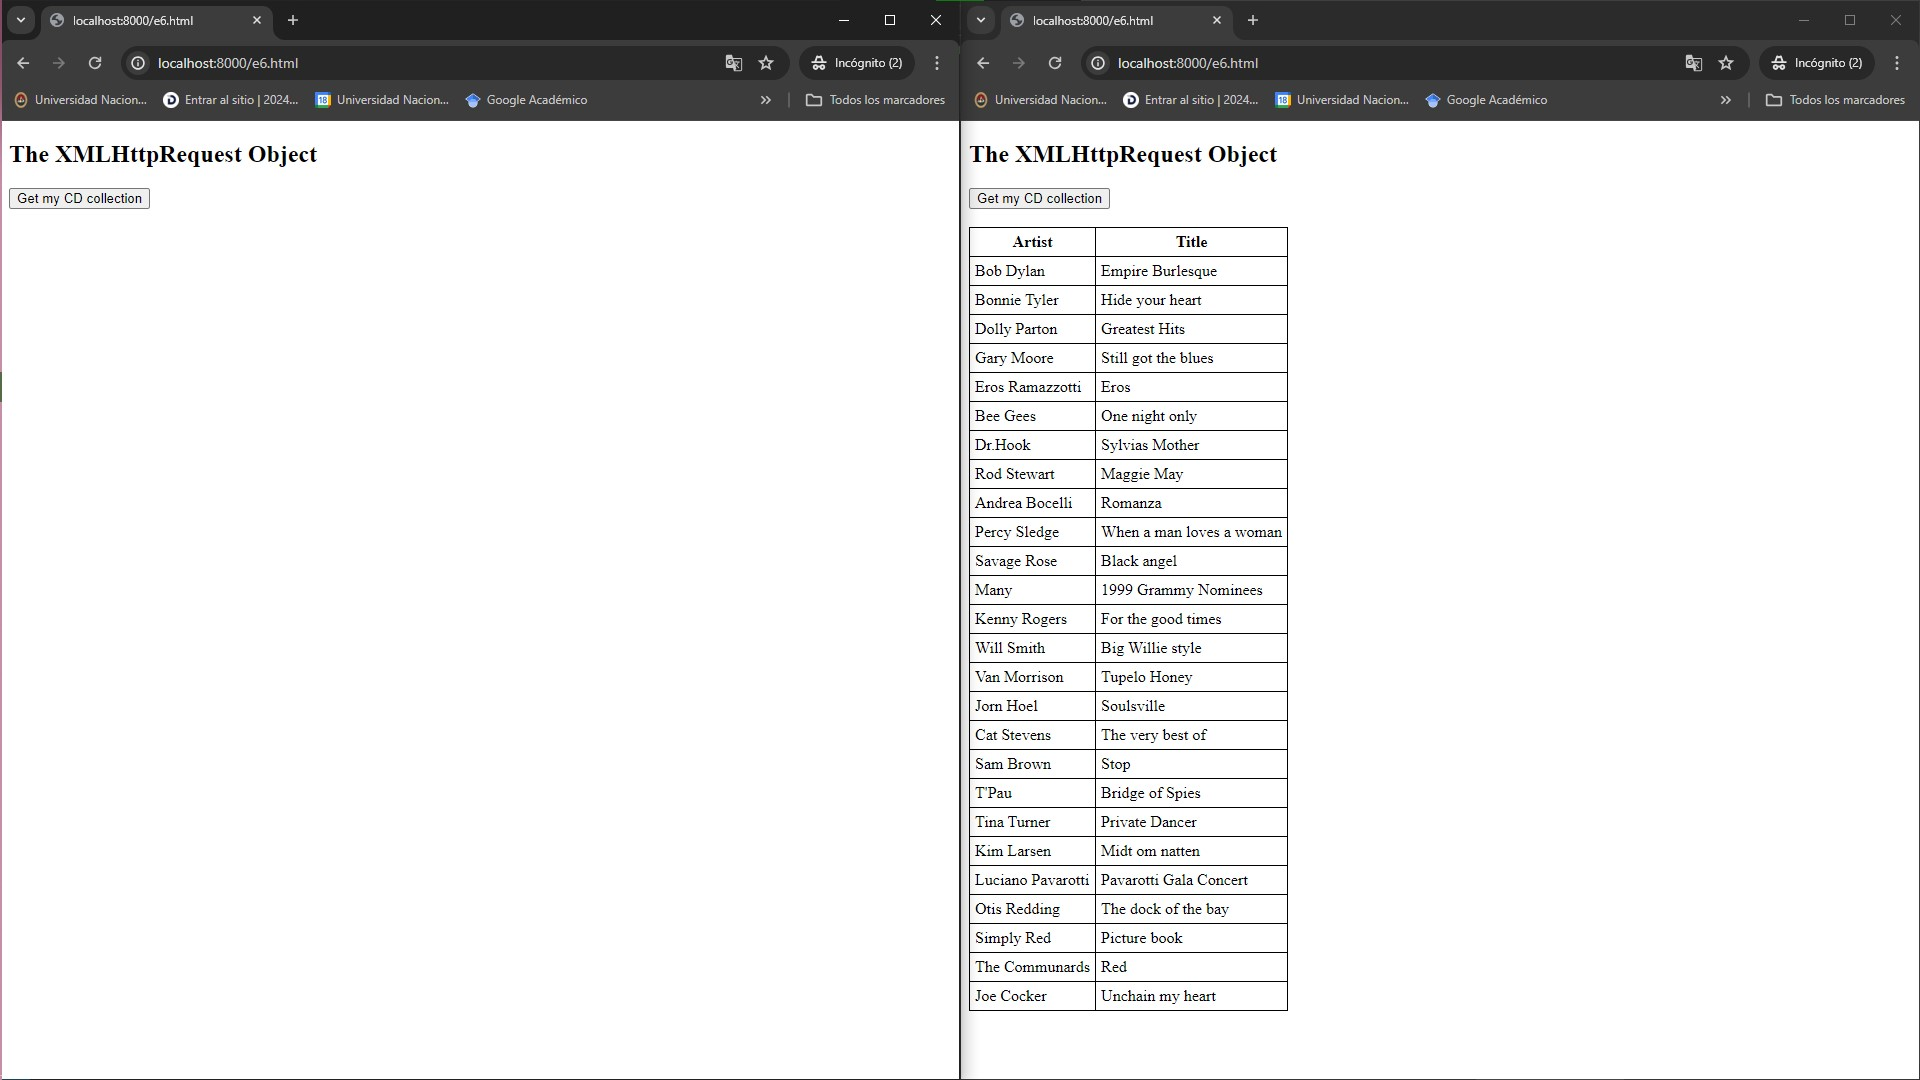
\includegraphics[width=0.7\textwidth]{img/ex6.jpg}
    \caption{Obtener informacion a travez de Ajax de un archivo XML}
    \end{figure}

\begin{figure}[H]
  \centering
  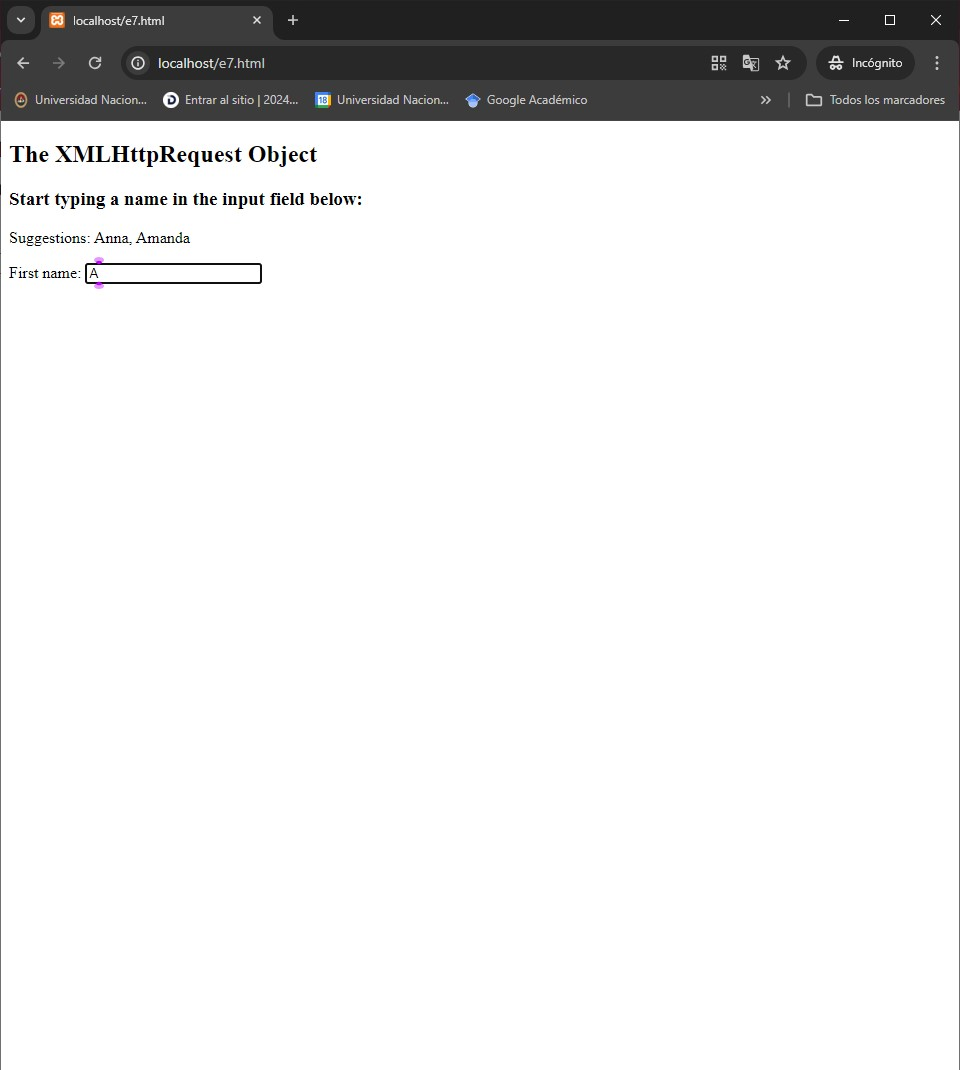
\includegraphics[width=0.5\textwidth]{img/ex7.jpg}
  \caption{Comunicacion entre un servidor web y una pagina web mientras se ingresan datos}
  \end{figure}

\begin{figure}[H]
  \centering
  
\includegraphics[width=0.7\textwidth]{img/ex8.jpg}
  \caption{Obtener informacion de una base de datos usando Ajax}
  \end{figure}

\begin{figure}[H]
  \centering
  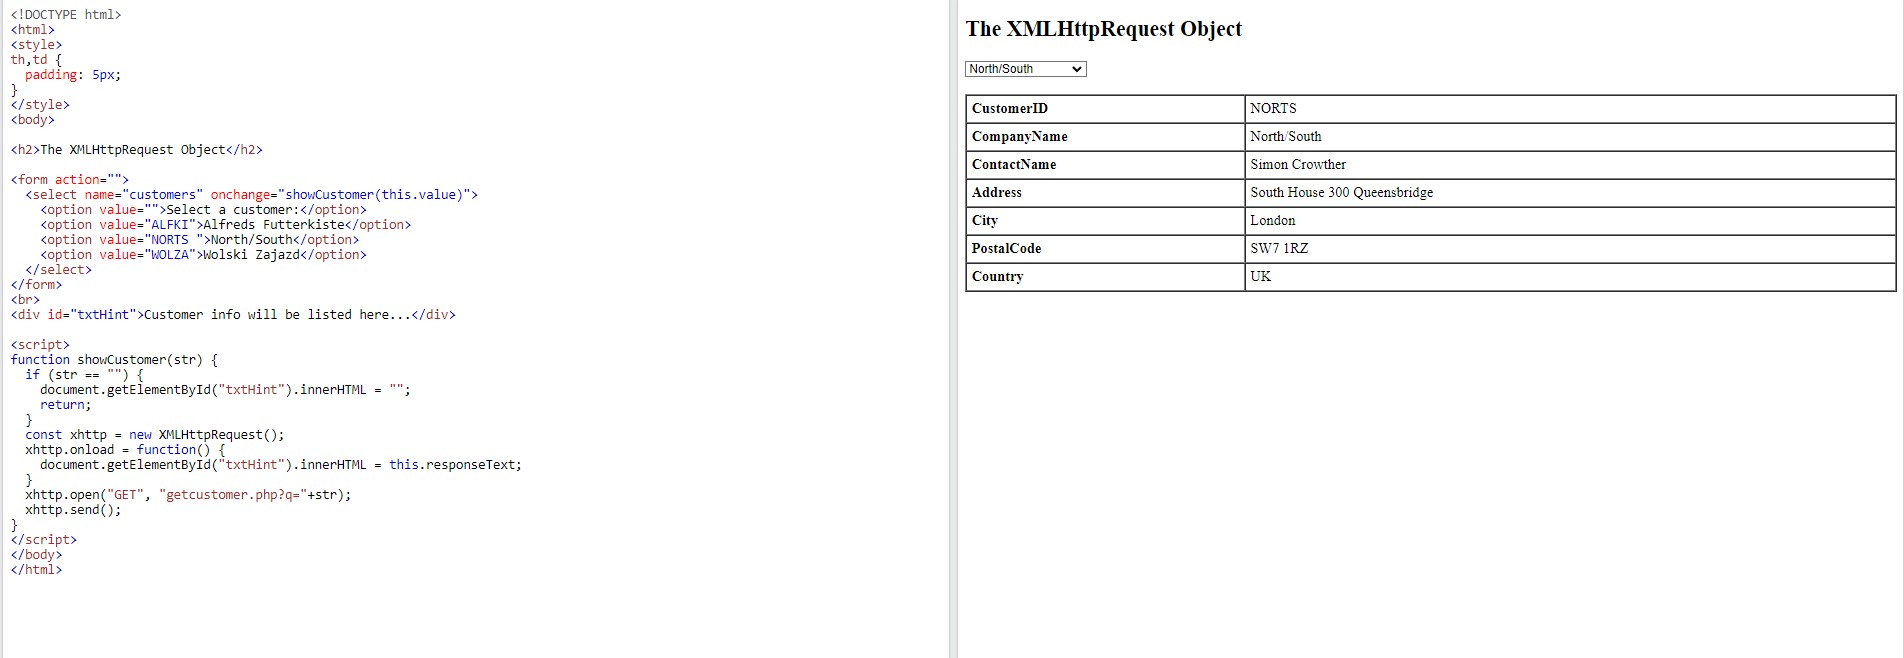
\includegraphics[width=0.7\textwidth]{img/ex9.jpg}
  \caption{Mostrando datos en una tabal HTML}
  \end{figure}

\begin{figure}[H]
    \centering
    
\includegraphics[width=0.5\textwidth]{img/ex10.jpg}
    \caption{ Pidiendo informacion de la base de datos}
    \end{figure}

\begin{figure}[H]
  \centering
  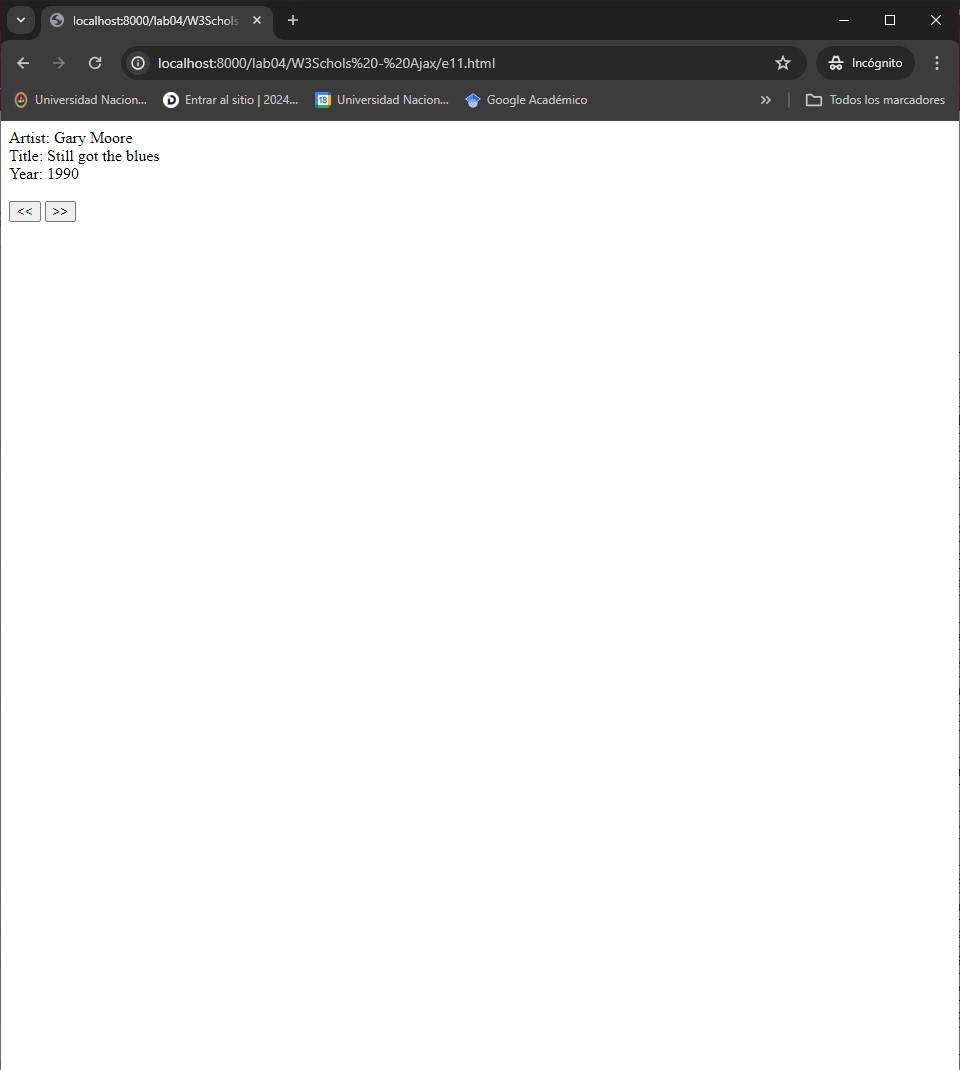
\includegraphics[width=0.5\textwidth]{img/ex11.jpg}
  \caption{Recorriendo la informacion de la base de datos}
  \end{figure}

\begin{figure}[H]
  \centering
  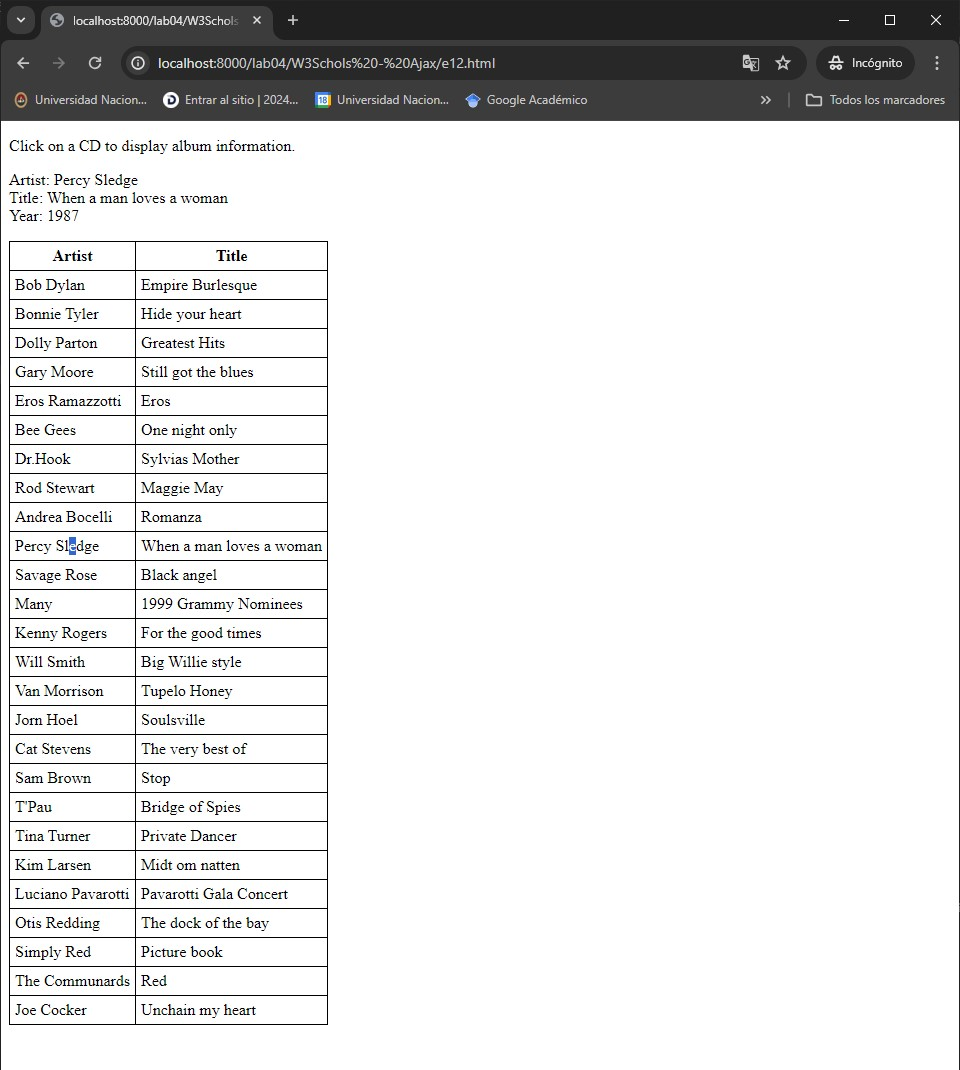
\includegraphics[width=0.5\textwidth]{img/ex12.jpg}
  \caption{Mostrar los elementos en una tabla HTML}
  \end{figure}
\section{Los 8 ejercicios JavaScript con Ajax y Google Chart}
En el priemr ejercicio tenemos una función de JavaScript llamada listRegions esta función recibe un arreglo de datos como parámetro y actualiza el contenido de un elemento HTML identificado por el id 'result'. Primero, borra cualquier contenido previo dentro de este elemento. Luego, itera sobre cada elemento del arreglo de datos. Para cada elemento, imprime el valor de la propiedad 'region' en la consola del navegador y crea un nuevo elemento de lista (li) con este valor como contenido de texto. Finalmente, añade este elemento de lista como hijo del elemento 'result' en el documento HTML.
\begin{figure}[H]
  \centering
  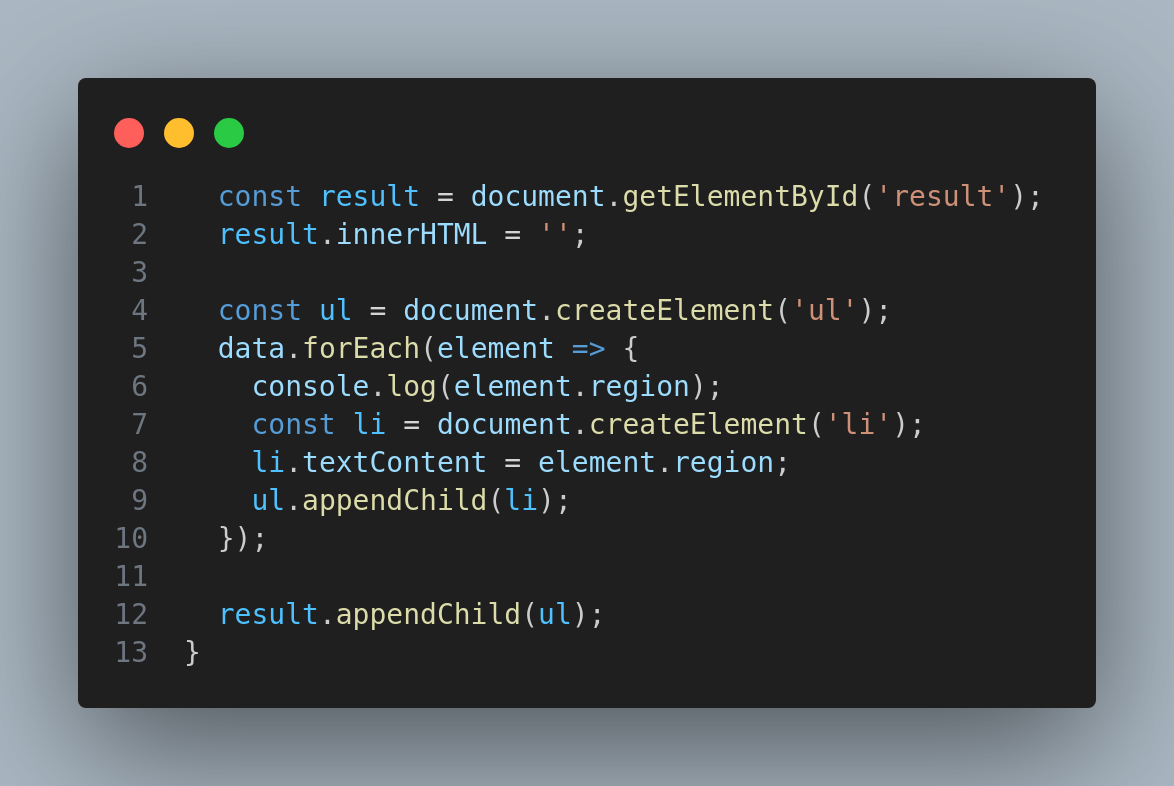
\includegraphics[width=1.0\textwidth]{img/1_js.png}
  \caption{ejercicio1.js}
\end{figure}
En el segundo ejercicio tenemos la función totalConfirmed toma un arreglo de datos como entrada y calcula el total de casos confirmados por región a partir de esos datos. Luego, genera una lista en el documento HTML que muestra cada región junto con su total de casos confirmados.
\begin{figure}[H]
  \centering
  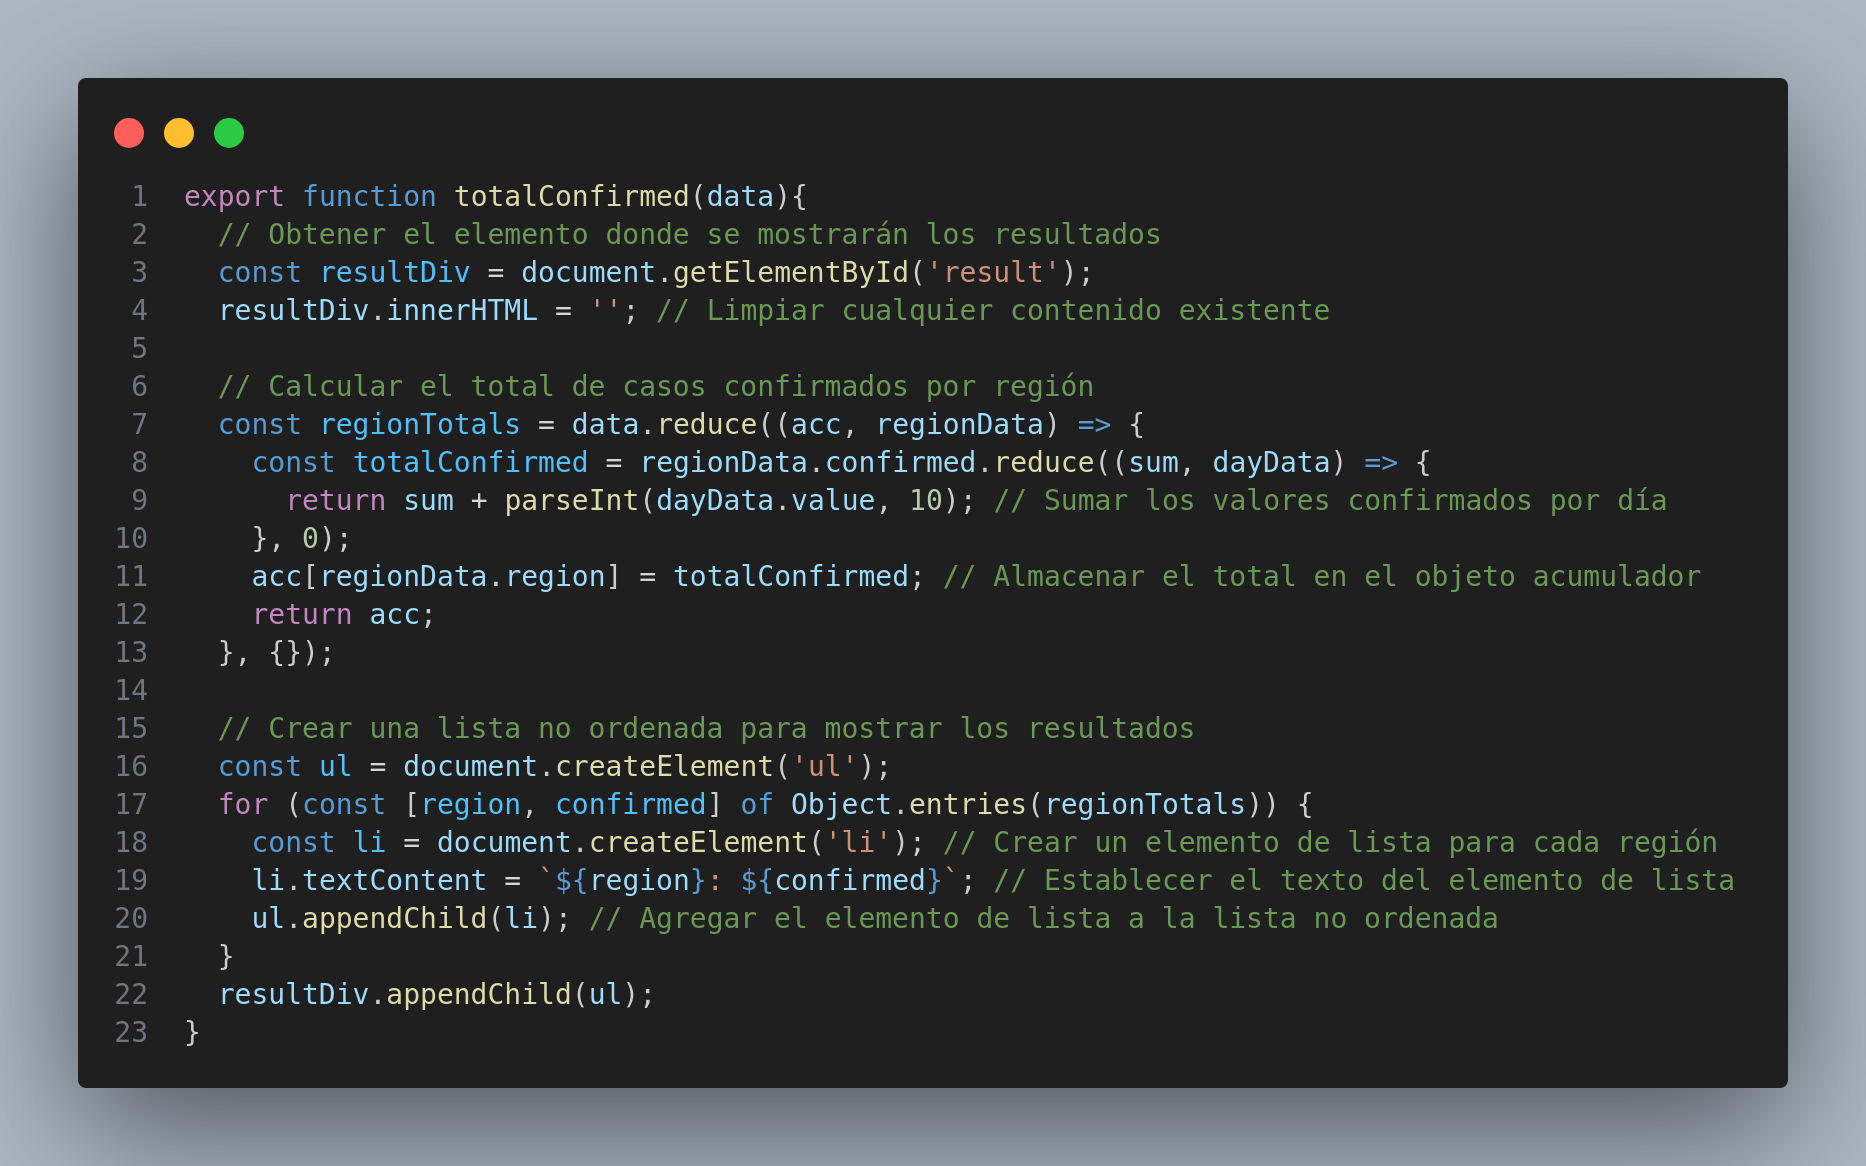
\includegraphics[width=1.0\textwidth]{img/2_js.png}
  \caption{ejercicio2.js}
\end{figure}
En el tercer ejercicio la función top10Regions también recibe un arreglo de datos y muestra los 10 principales regiones junto con sus totales de casos confirmados en orden descendente en el documento HTML. Comienza limpiando cualquier contenido previo dentro del elemento HTML identificado por el id 'result'. Luego, calcula el total de casos confirmados por región, similar a la función totalConfirmed. Después, ordena las regiones por el número total de casos confirmados en orden descendente y toma las primeras 10. Finalmente, crea una lista no ordenada en el documento HTML para mostrar los resultados y agrega cada región junto con su total de casos confirmados como elementos de lista.

\begin{figure}[H]
  \centering
  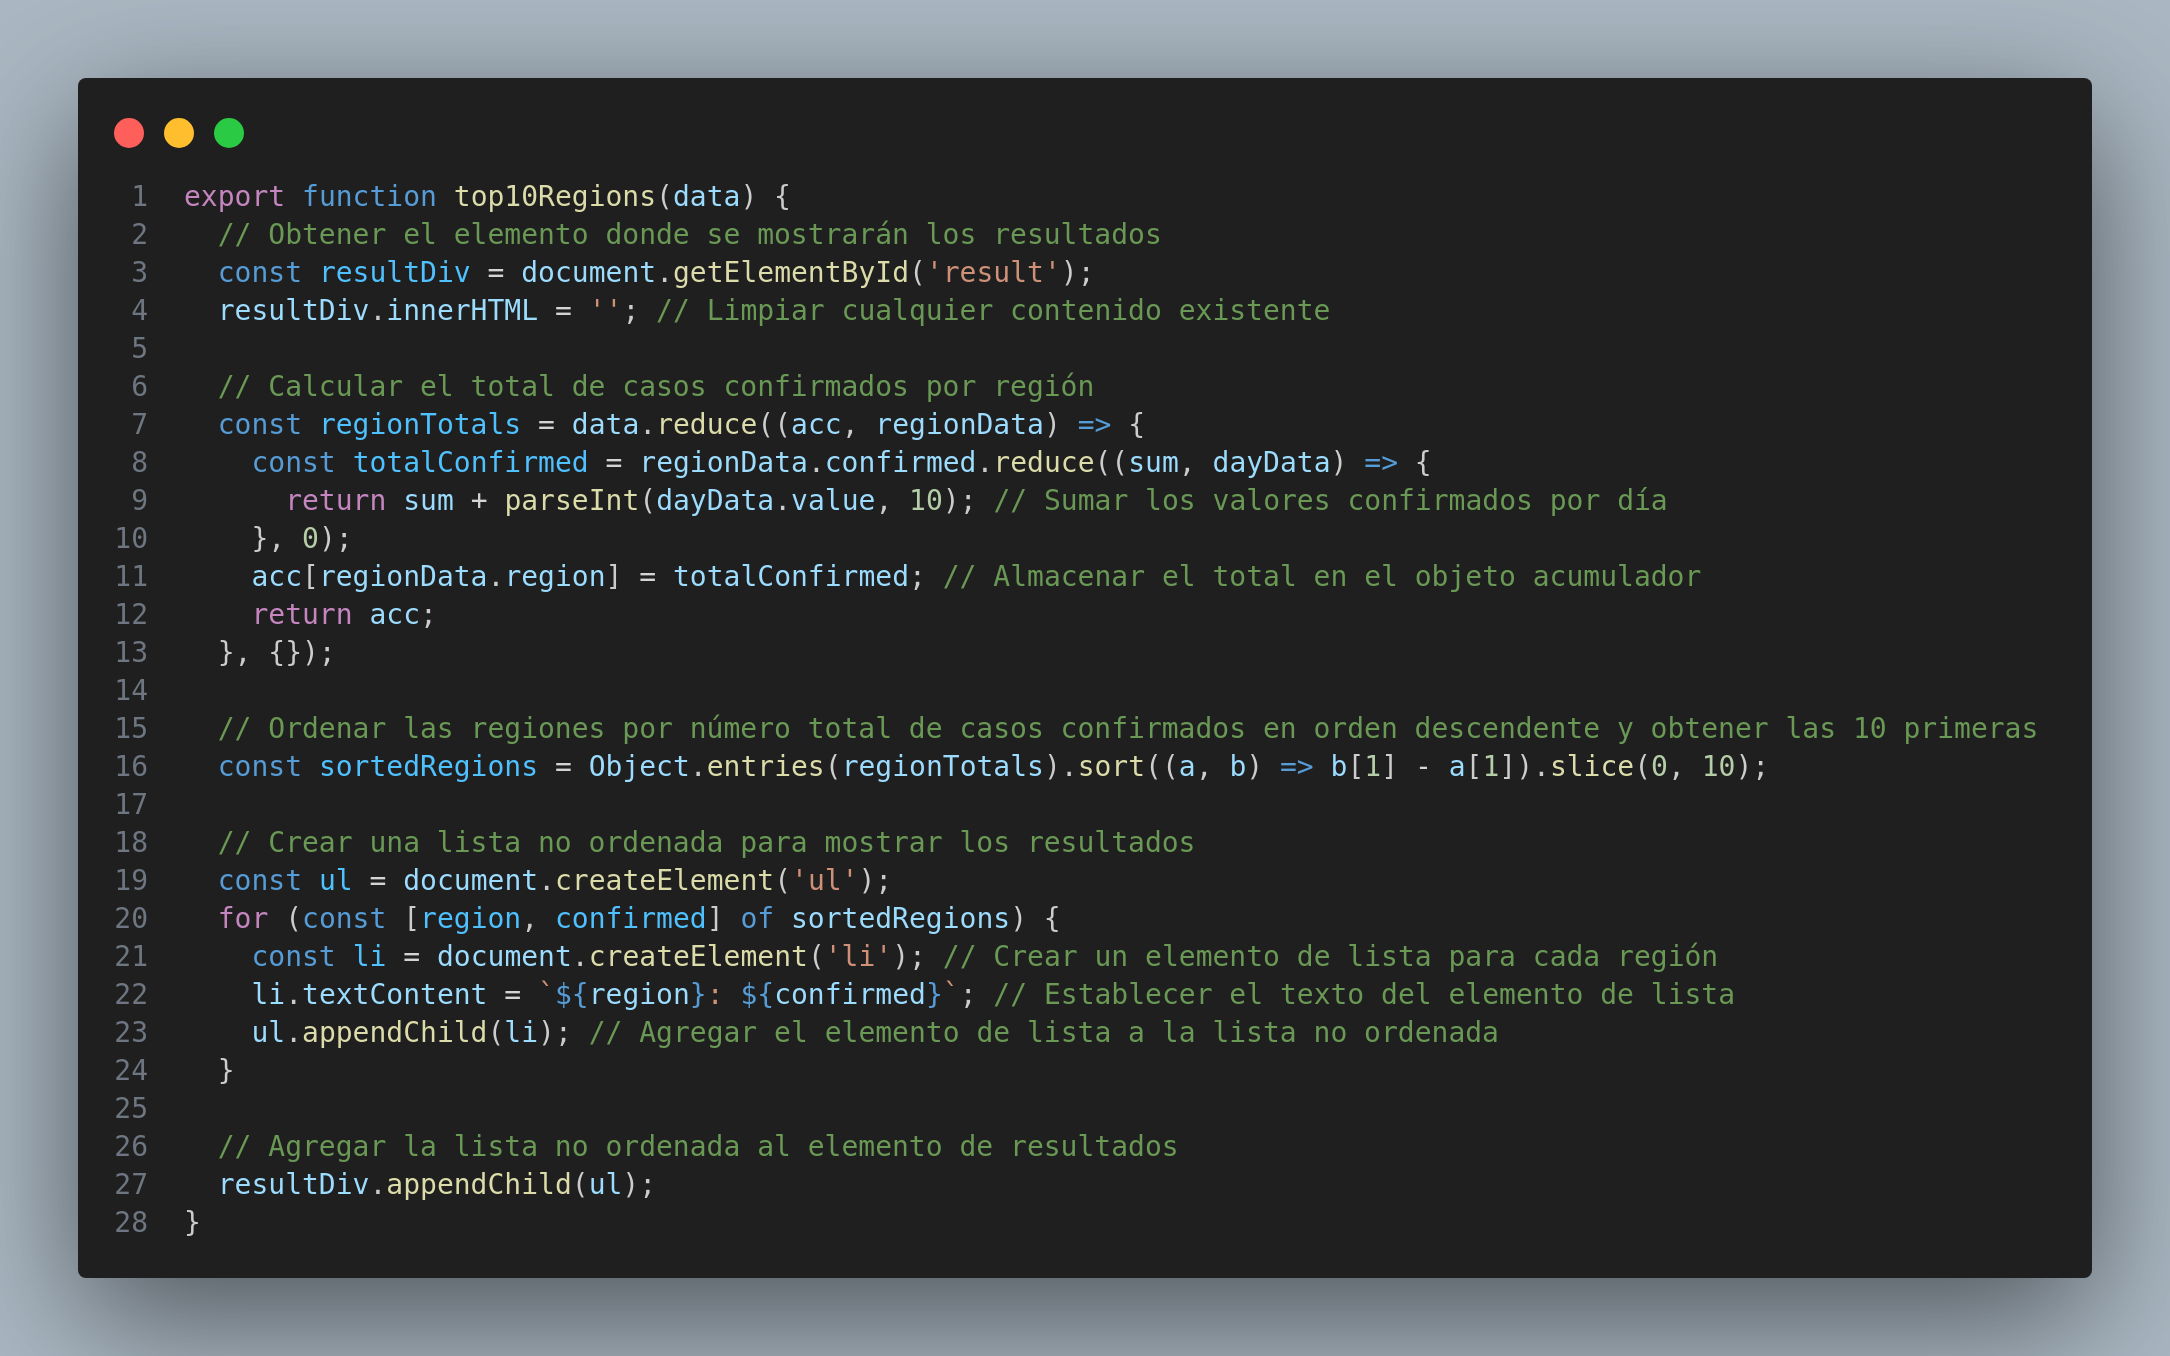
\includegraphics[width=1.0\textwidth]{img/3_js.png}
  \caption{ejercicio3.js}
\end{figure}

En el cuarto ejercicio la función arequipaInfected se encarga de visualizar los datos de infectados en la región de Arequipa a lo largo del tiempo. Comienza filtrando los datos para obtener solo la información relacionada con la región de Arequipa. Luego, crea una nueva tabla de datos de Google Visualization y agrega una columna para las fechas y columnas para cada región en Arequipa. Posteriormente, itera sobre las fechas y para cada fecha, crea una nueva fila y agrega los valores de infectados correspondientes a cada región en esa fecha. Establece opciones de configuración para el gráfico, como título, dimensiones y estilos de ejes, y finalmente, crea una instancia del gráfico de líneas de Google Visualization y lo dibuja en el elemento HTML con el ID "result".
\begin{figure}[H]
  \centering
  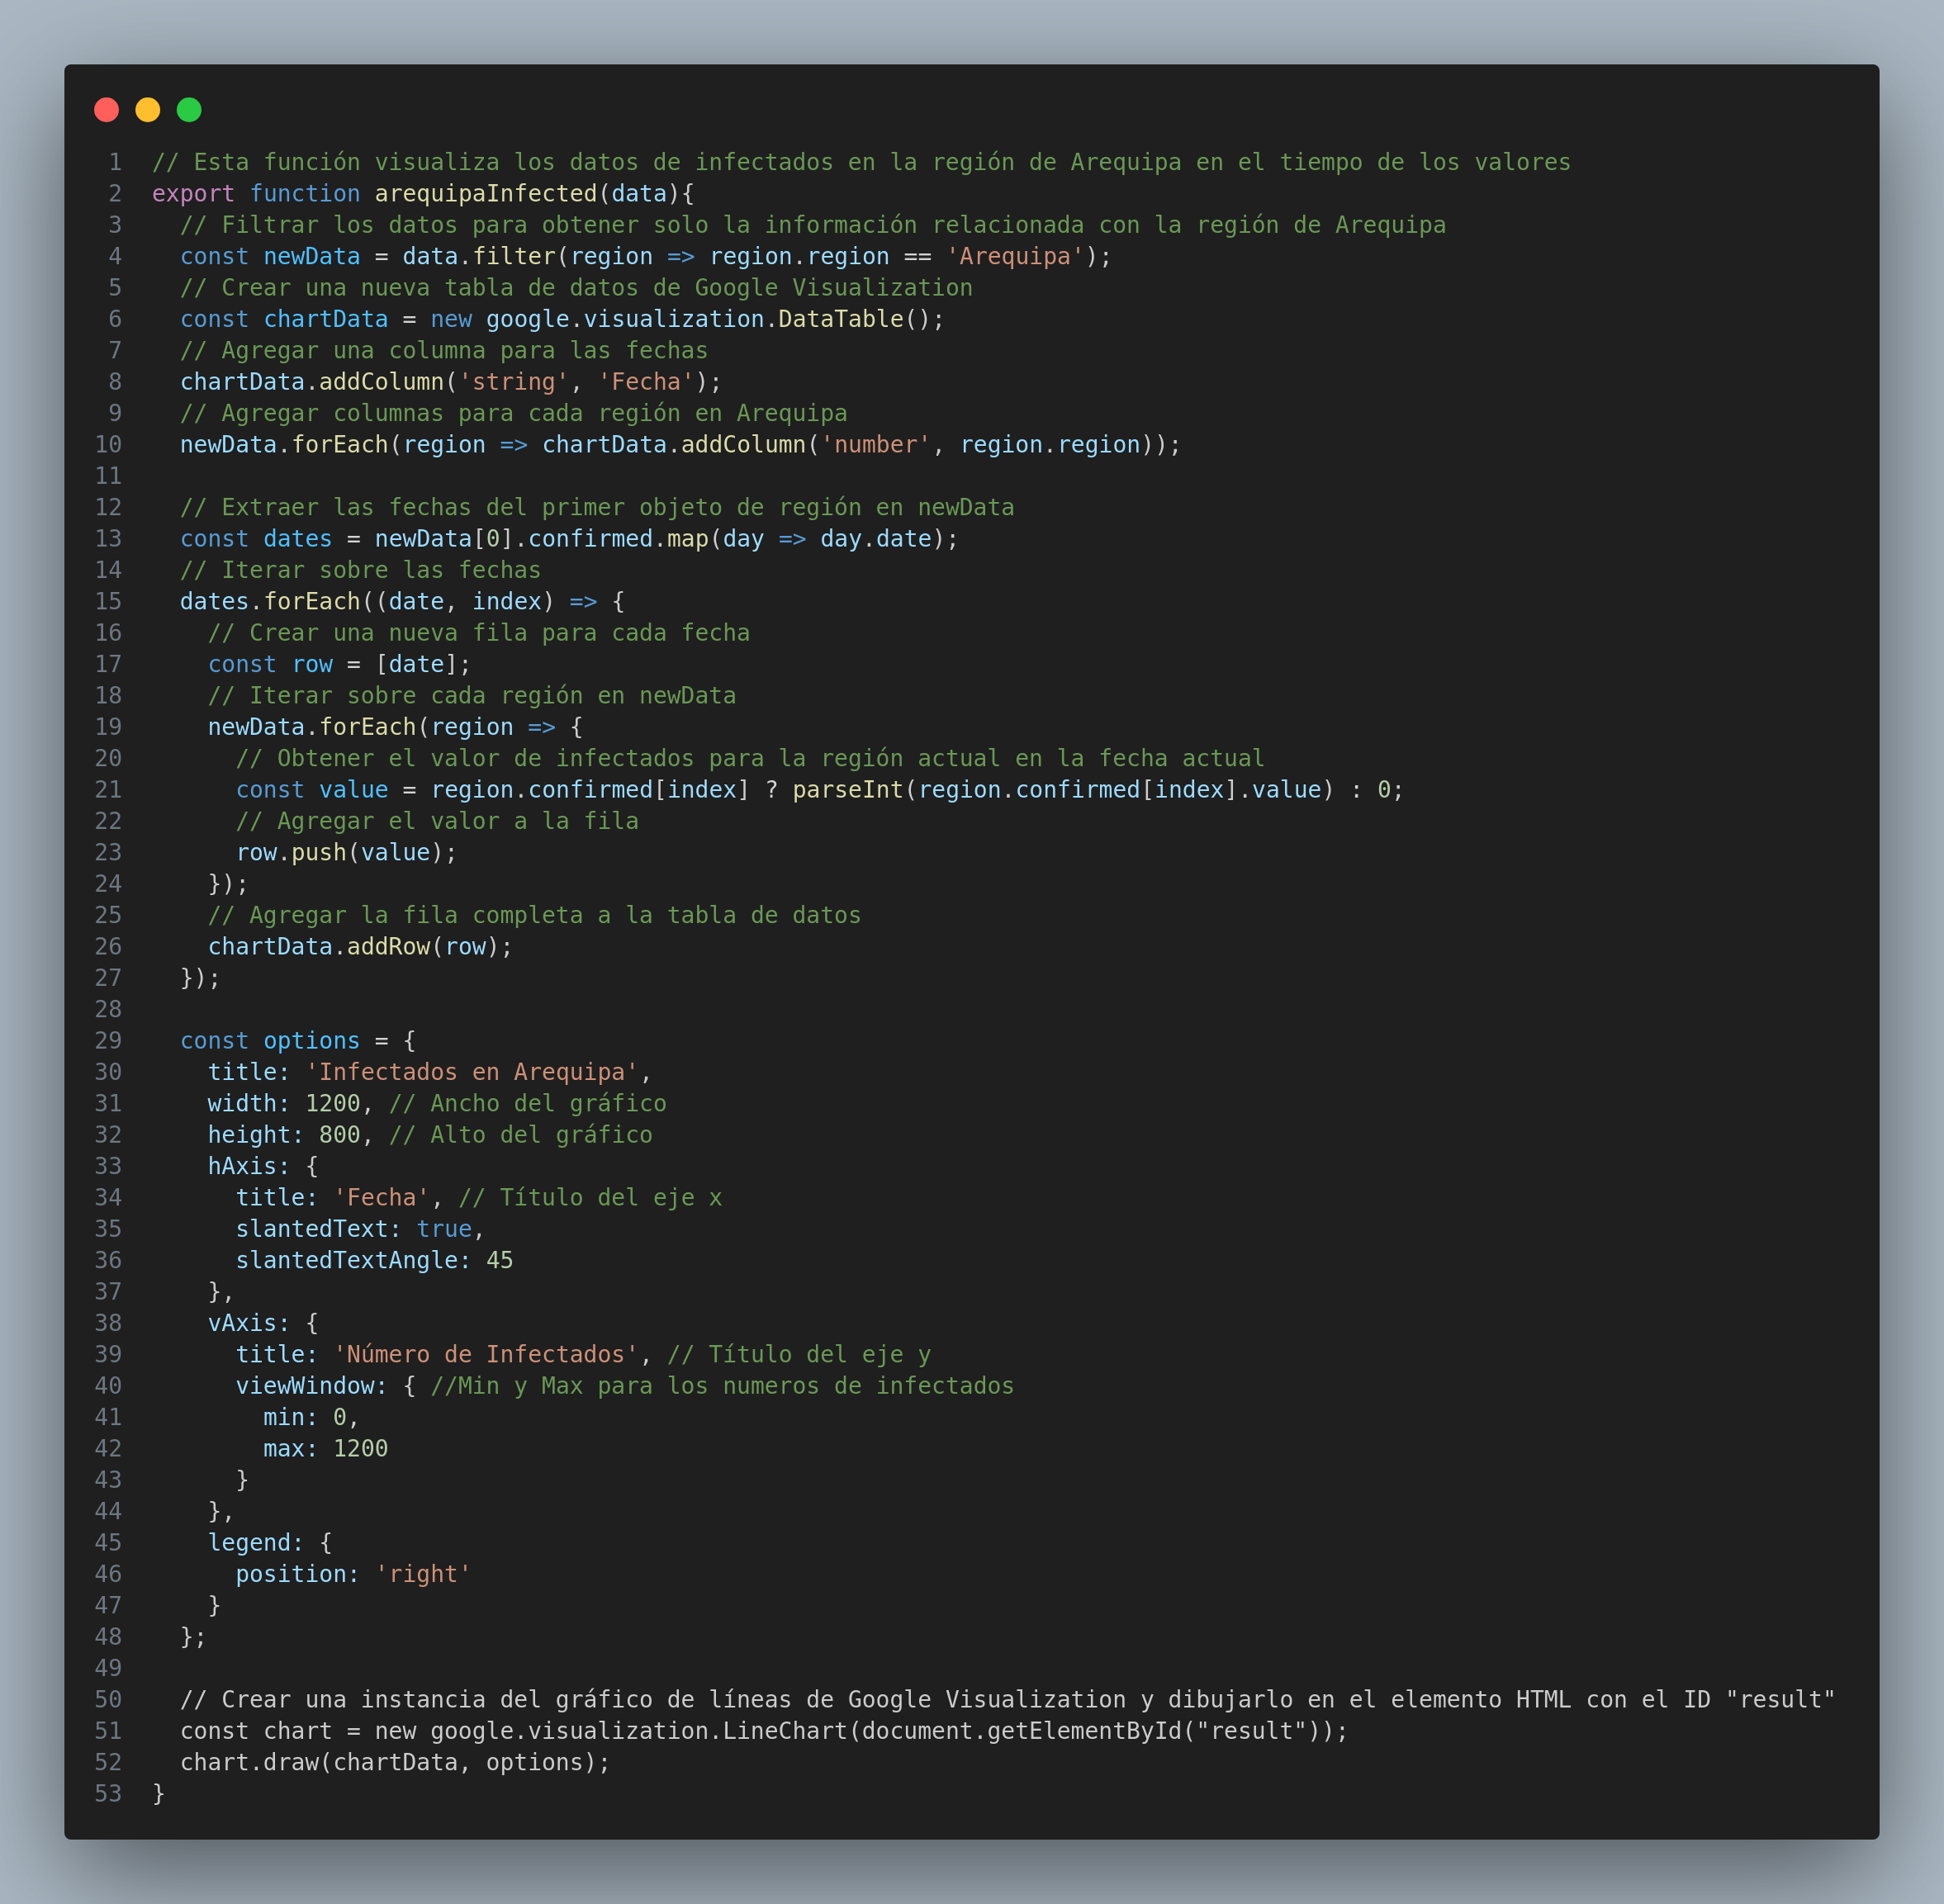
\includegraphics[width=1.0\textwidth]{img/4_js.png}
  \caption{ejercicio4.js}
\end{figure}
En el quinto ejercicio la función comparativeLineChart analiza datos sobre casos confirmados en todas las regiones y crea un gráfico de líneas que compara el crecimiento de estos casos a lo largo del tiempo. Para ello, primero filtra los datos para obtener información de todas las regiones disponibles. Luego, estructura estos datos en una tabla de Google Visualization, donde cada fila representa una fecha y cada columna representa una región, con los valores de casos confirmados en cada fecha. Se definen opciones para personalizar el aspecto del gráfico, como el título y los ejes x e y. Finalmente, utiliza la biblioteca de Google Visualization para dibujar el gráfico en un elemento HTML específico identificado por el ID "result".
\begin{figure}[H]
  \centering
  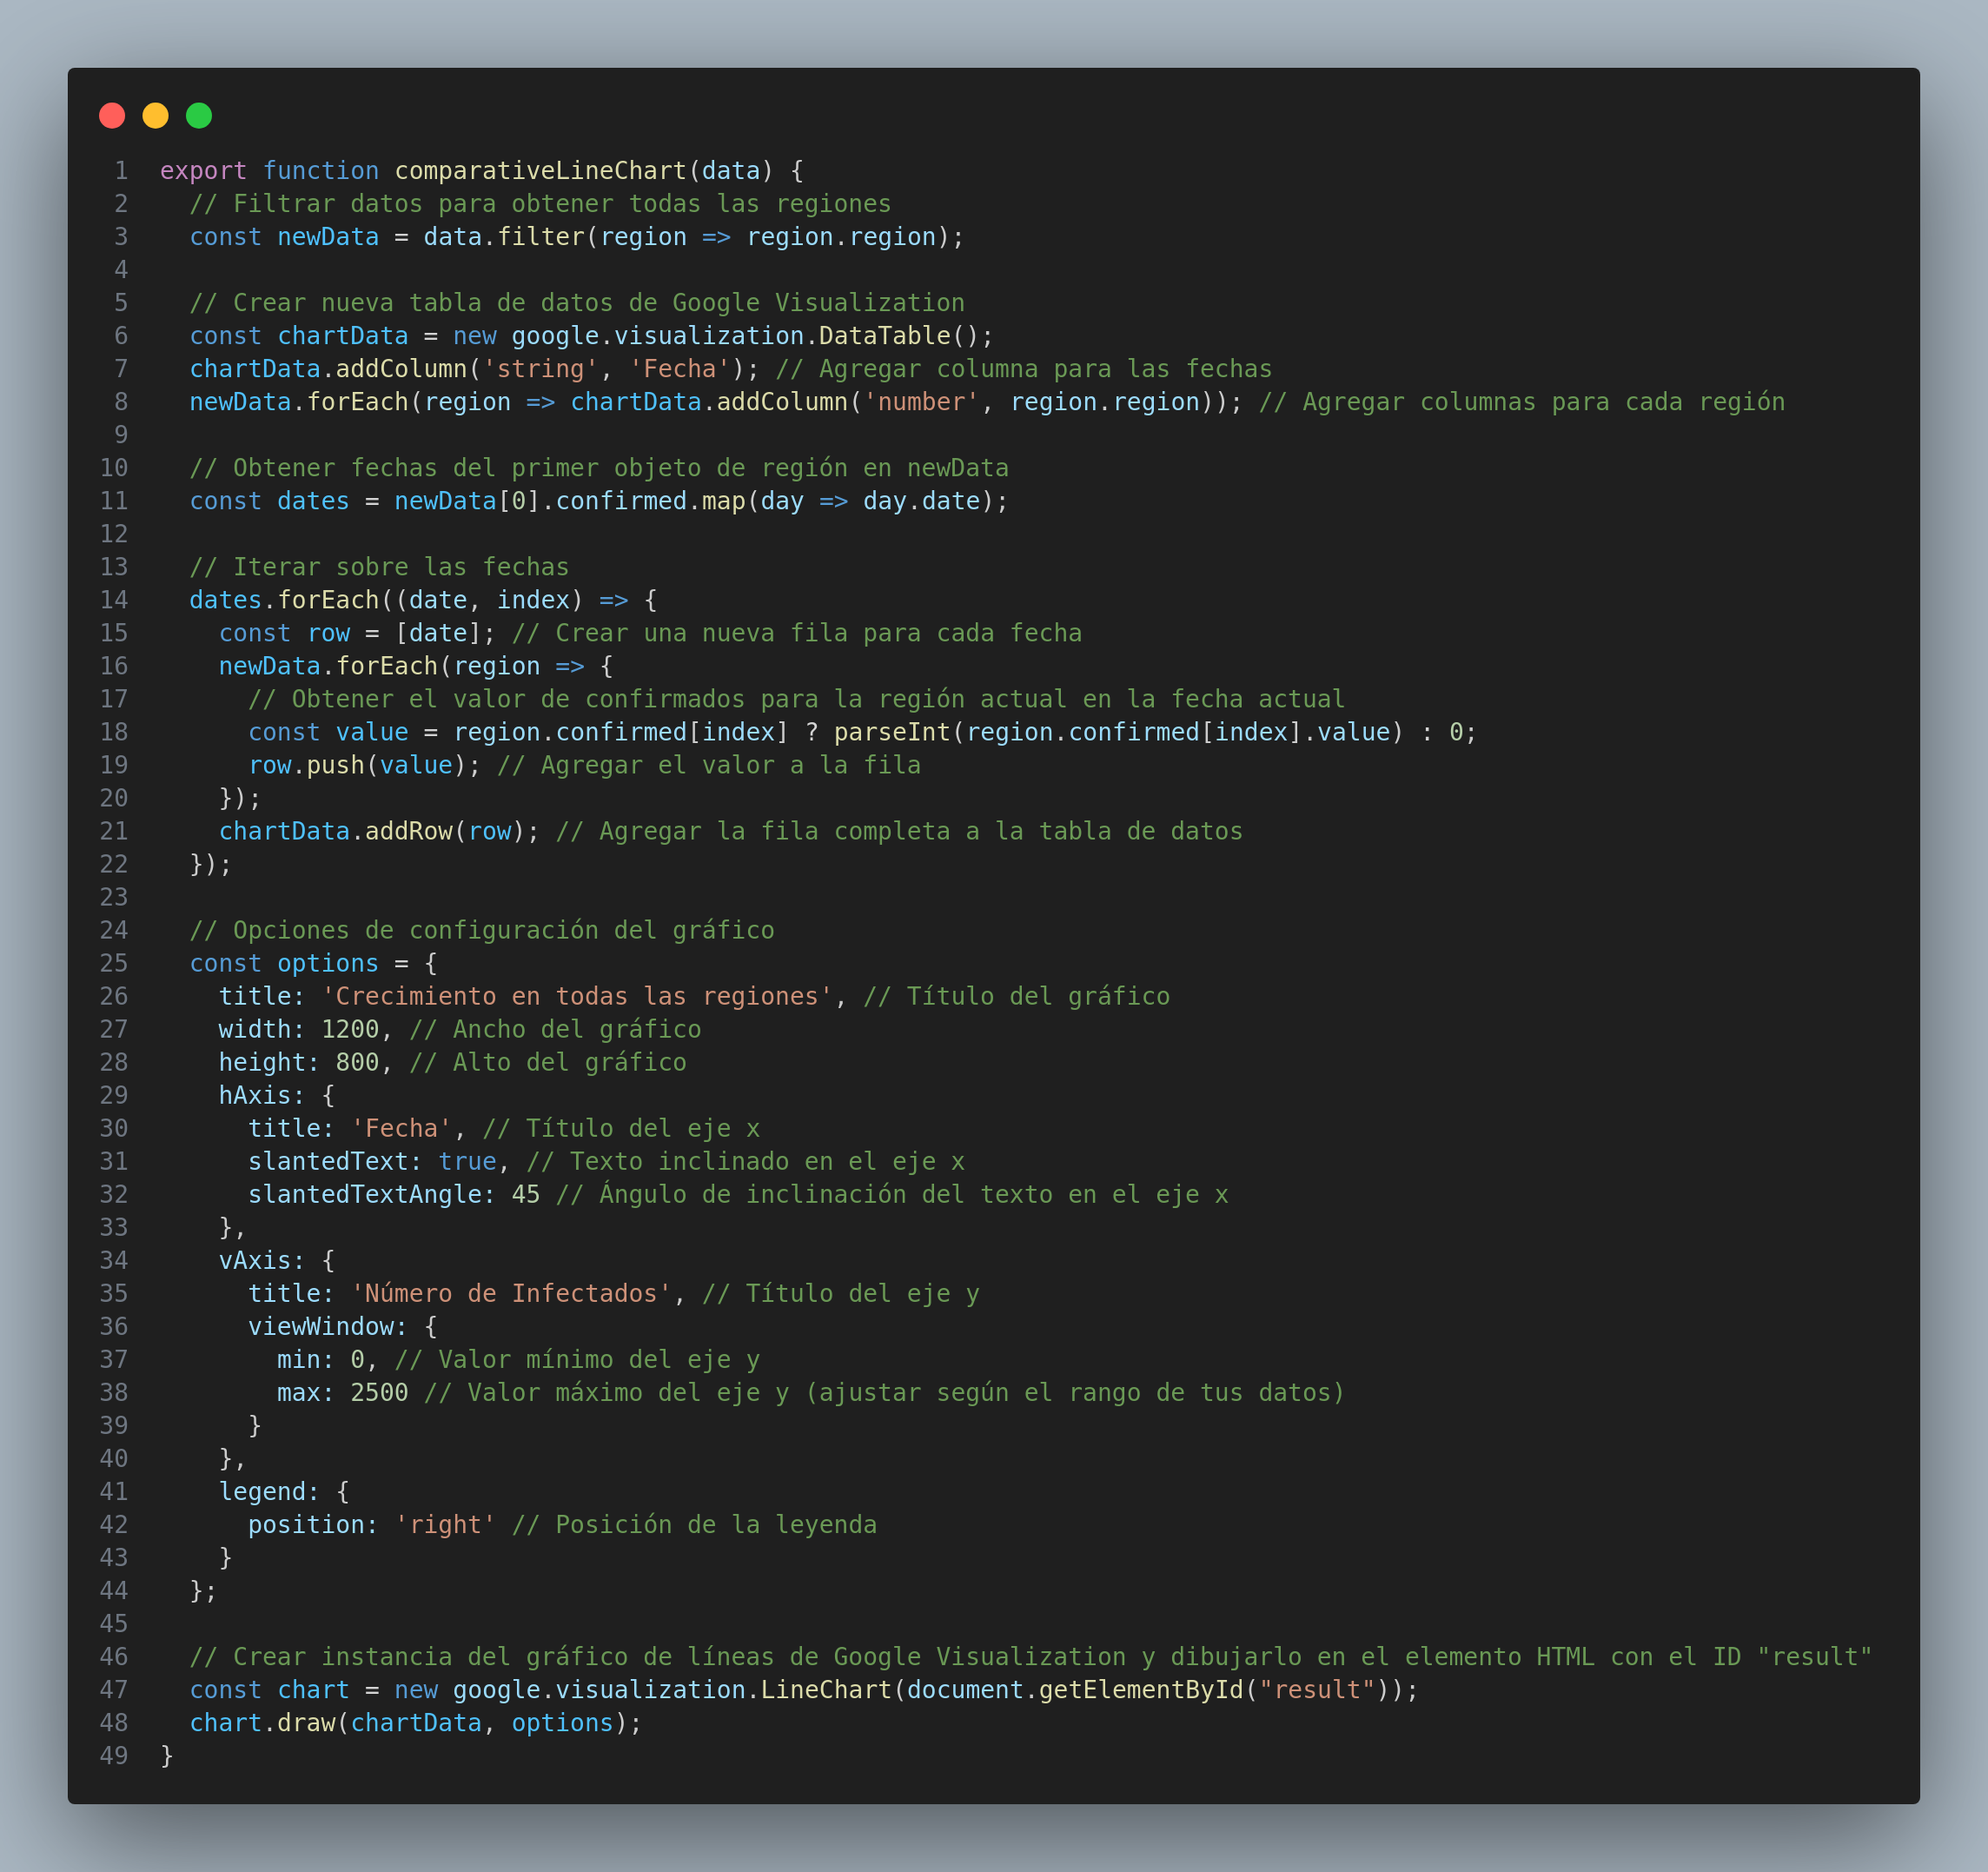
\includegraphics[width=1.0\textwidth]{img/5_js.png}
  \caption{ejercicio5.js}
\end{figure}
En el sexto ejercicio tenemos la función growthWithoutLimaCallao realiza un análisis similar a la función comparativeLineChart, pero excluye las regiones de Lima y Callao. Comienza filtrando los datos para excluir estas dos regiones y luego estructura los datos restantes en una tabla de Google Visualization. Posteriormente, crea un gráfico de líneas que muestra el crecimiento de casos confirmados para las regiones restantes a lo largo del tiempo. Se definen opciones de configuración para el gráfico, como el título y los ejes x e y. Finalmente, utiliza la biblioteca de Google Visualization para dibujar el gráfico en un elemento HTML específico identificado por el ID "result".
\begin{figure}[H]
  \centering
  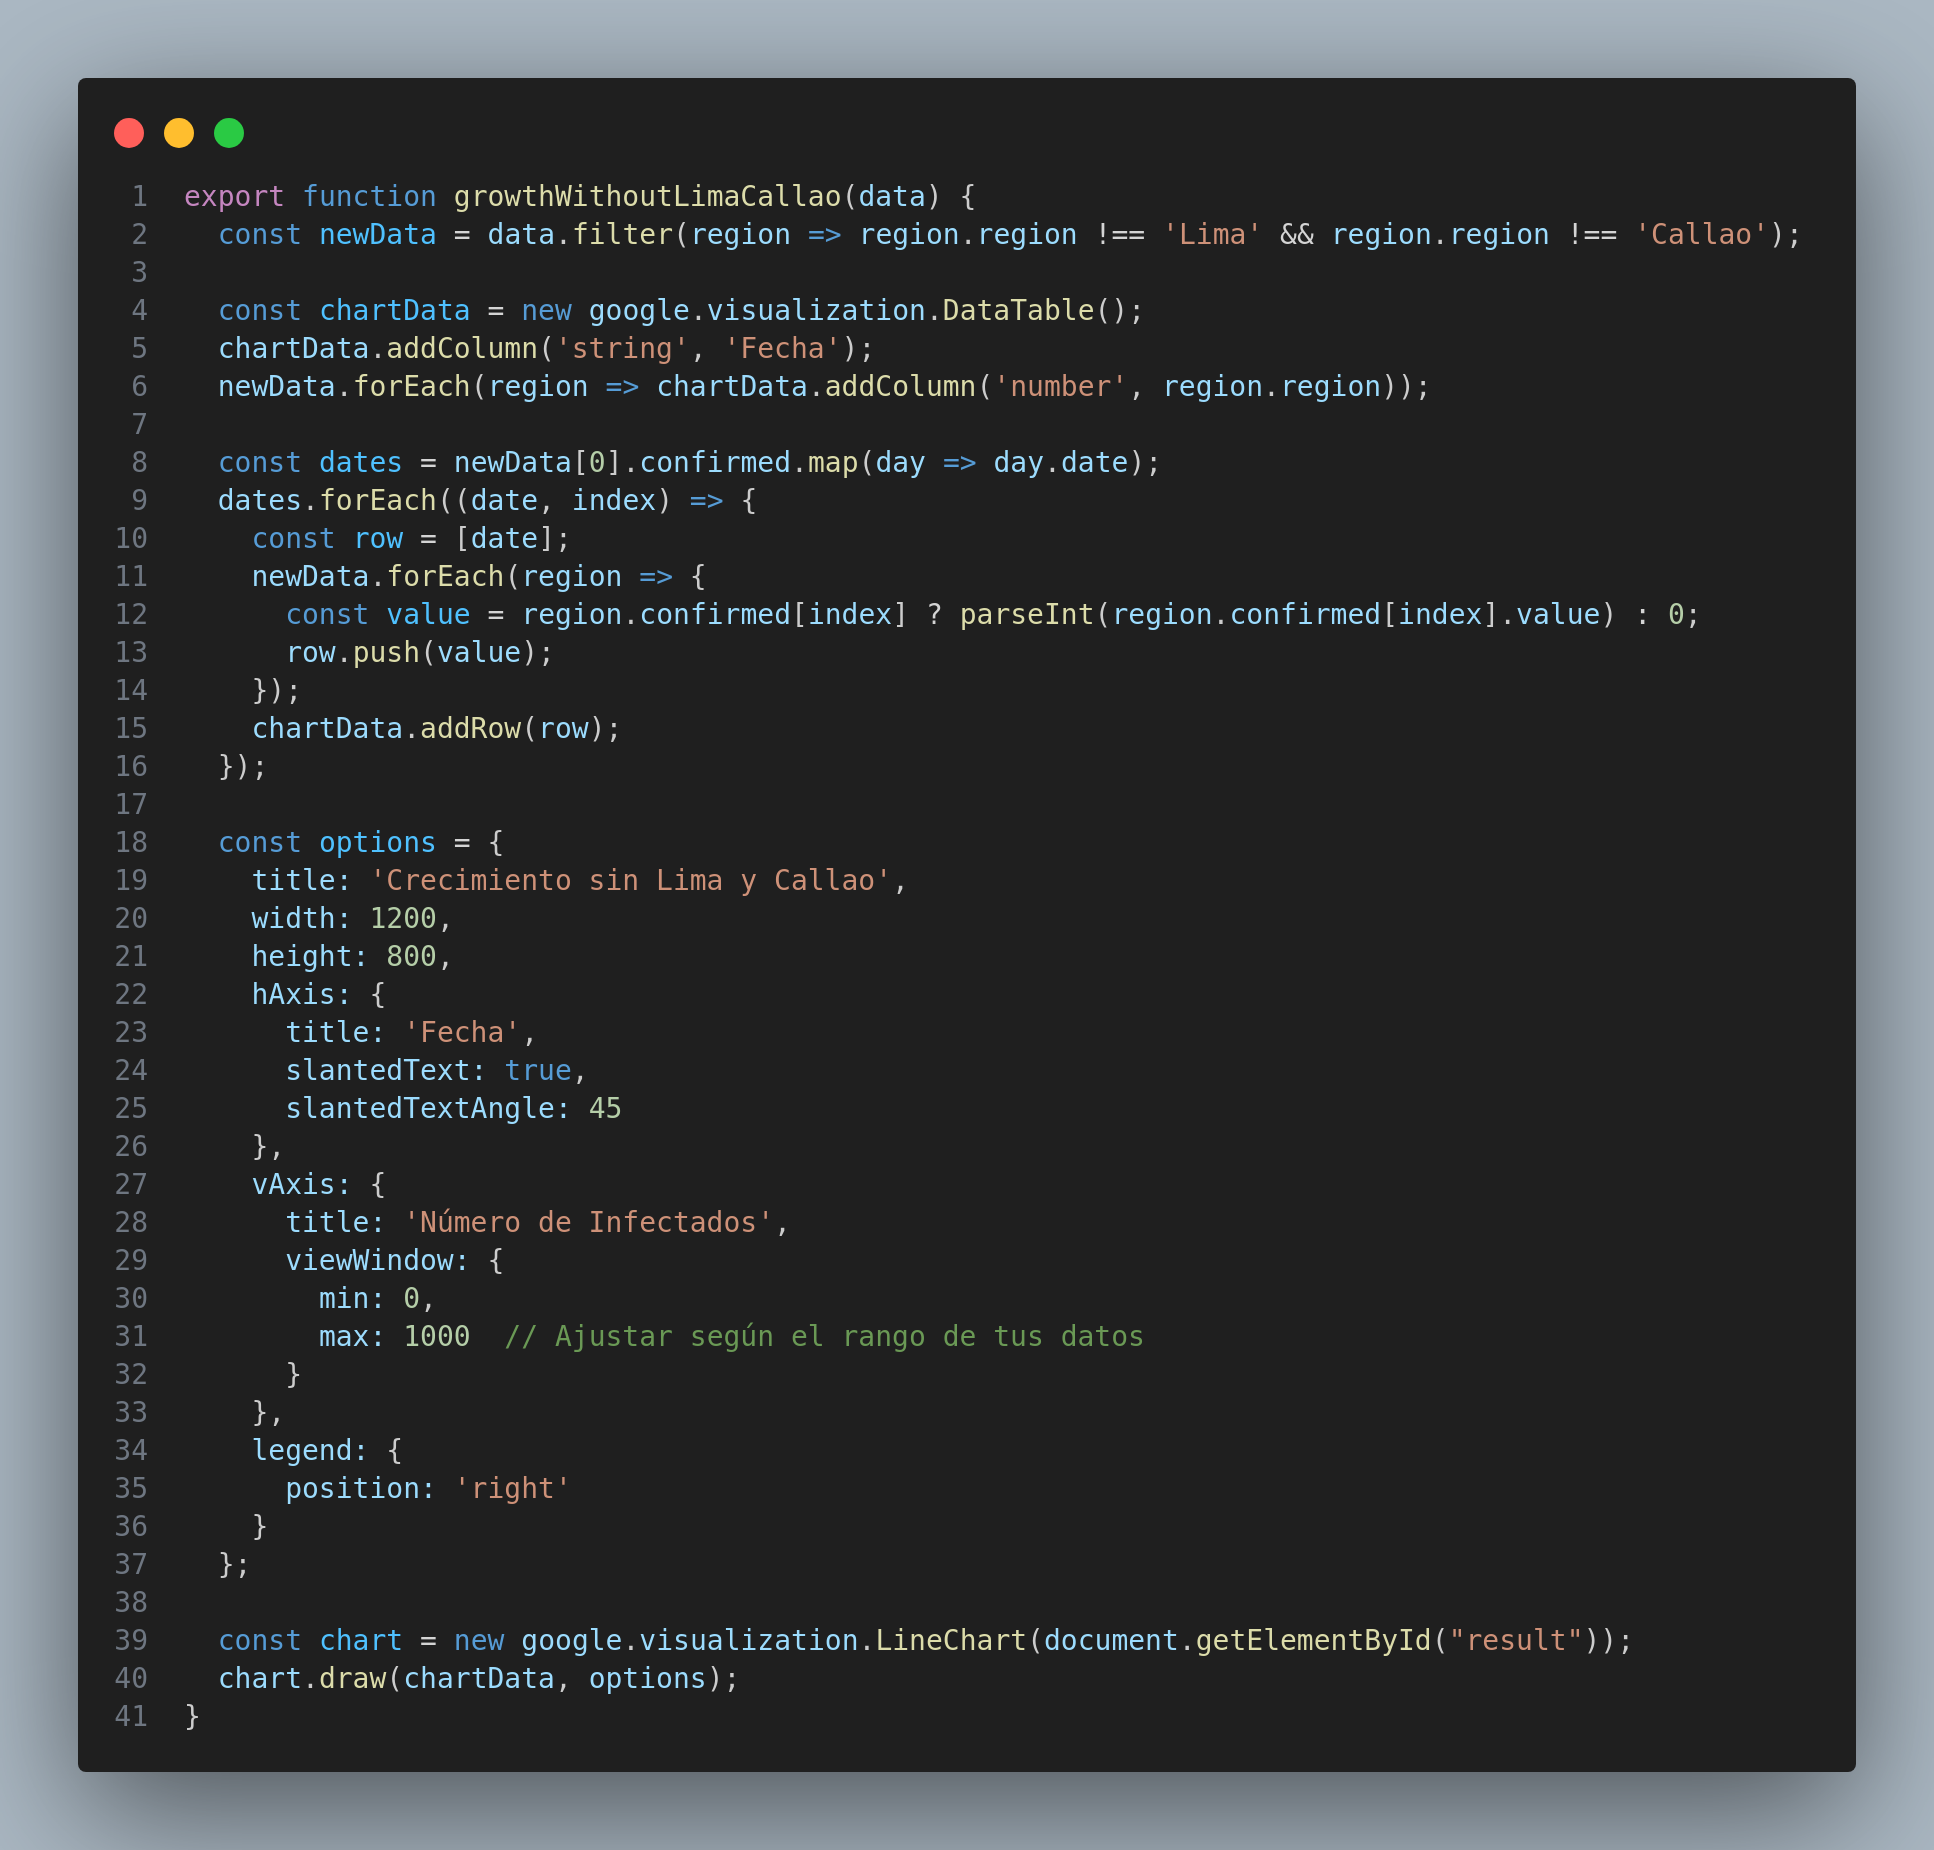
\includegraphics[width=1.0\textwidth]{img/6_js.png}
  \caption{ejercicio6.js}
\end{figure}
En el septimo ejercicio la función compareRegions compara el crecimiento de casos confirmados entre múltiples regiones utilizando una estructura similar a las funciones anteriores, pero sin excluir regiones específicas. Comienza creando una tabla de datos de Google Visualization con columnas para las fechas y cada región. Luego, añade filas de datos asumiendo que todas las regiones tienen las mismas fechas. Finalmente, genera un gráfico de líneas con opciones de configuración como título y ejes, mostrando la comparación en un elemento HTML con ID "result". Esta función simplifica el proceso de comparación al evitar la necesidad de excluir regiones específicas en el código.
\begin{figure}[H]
  \centering
  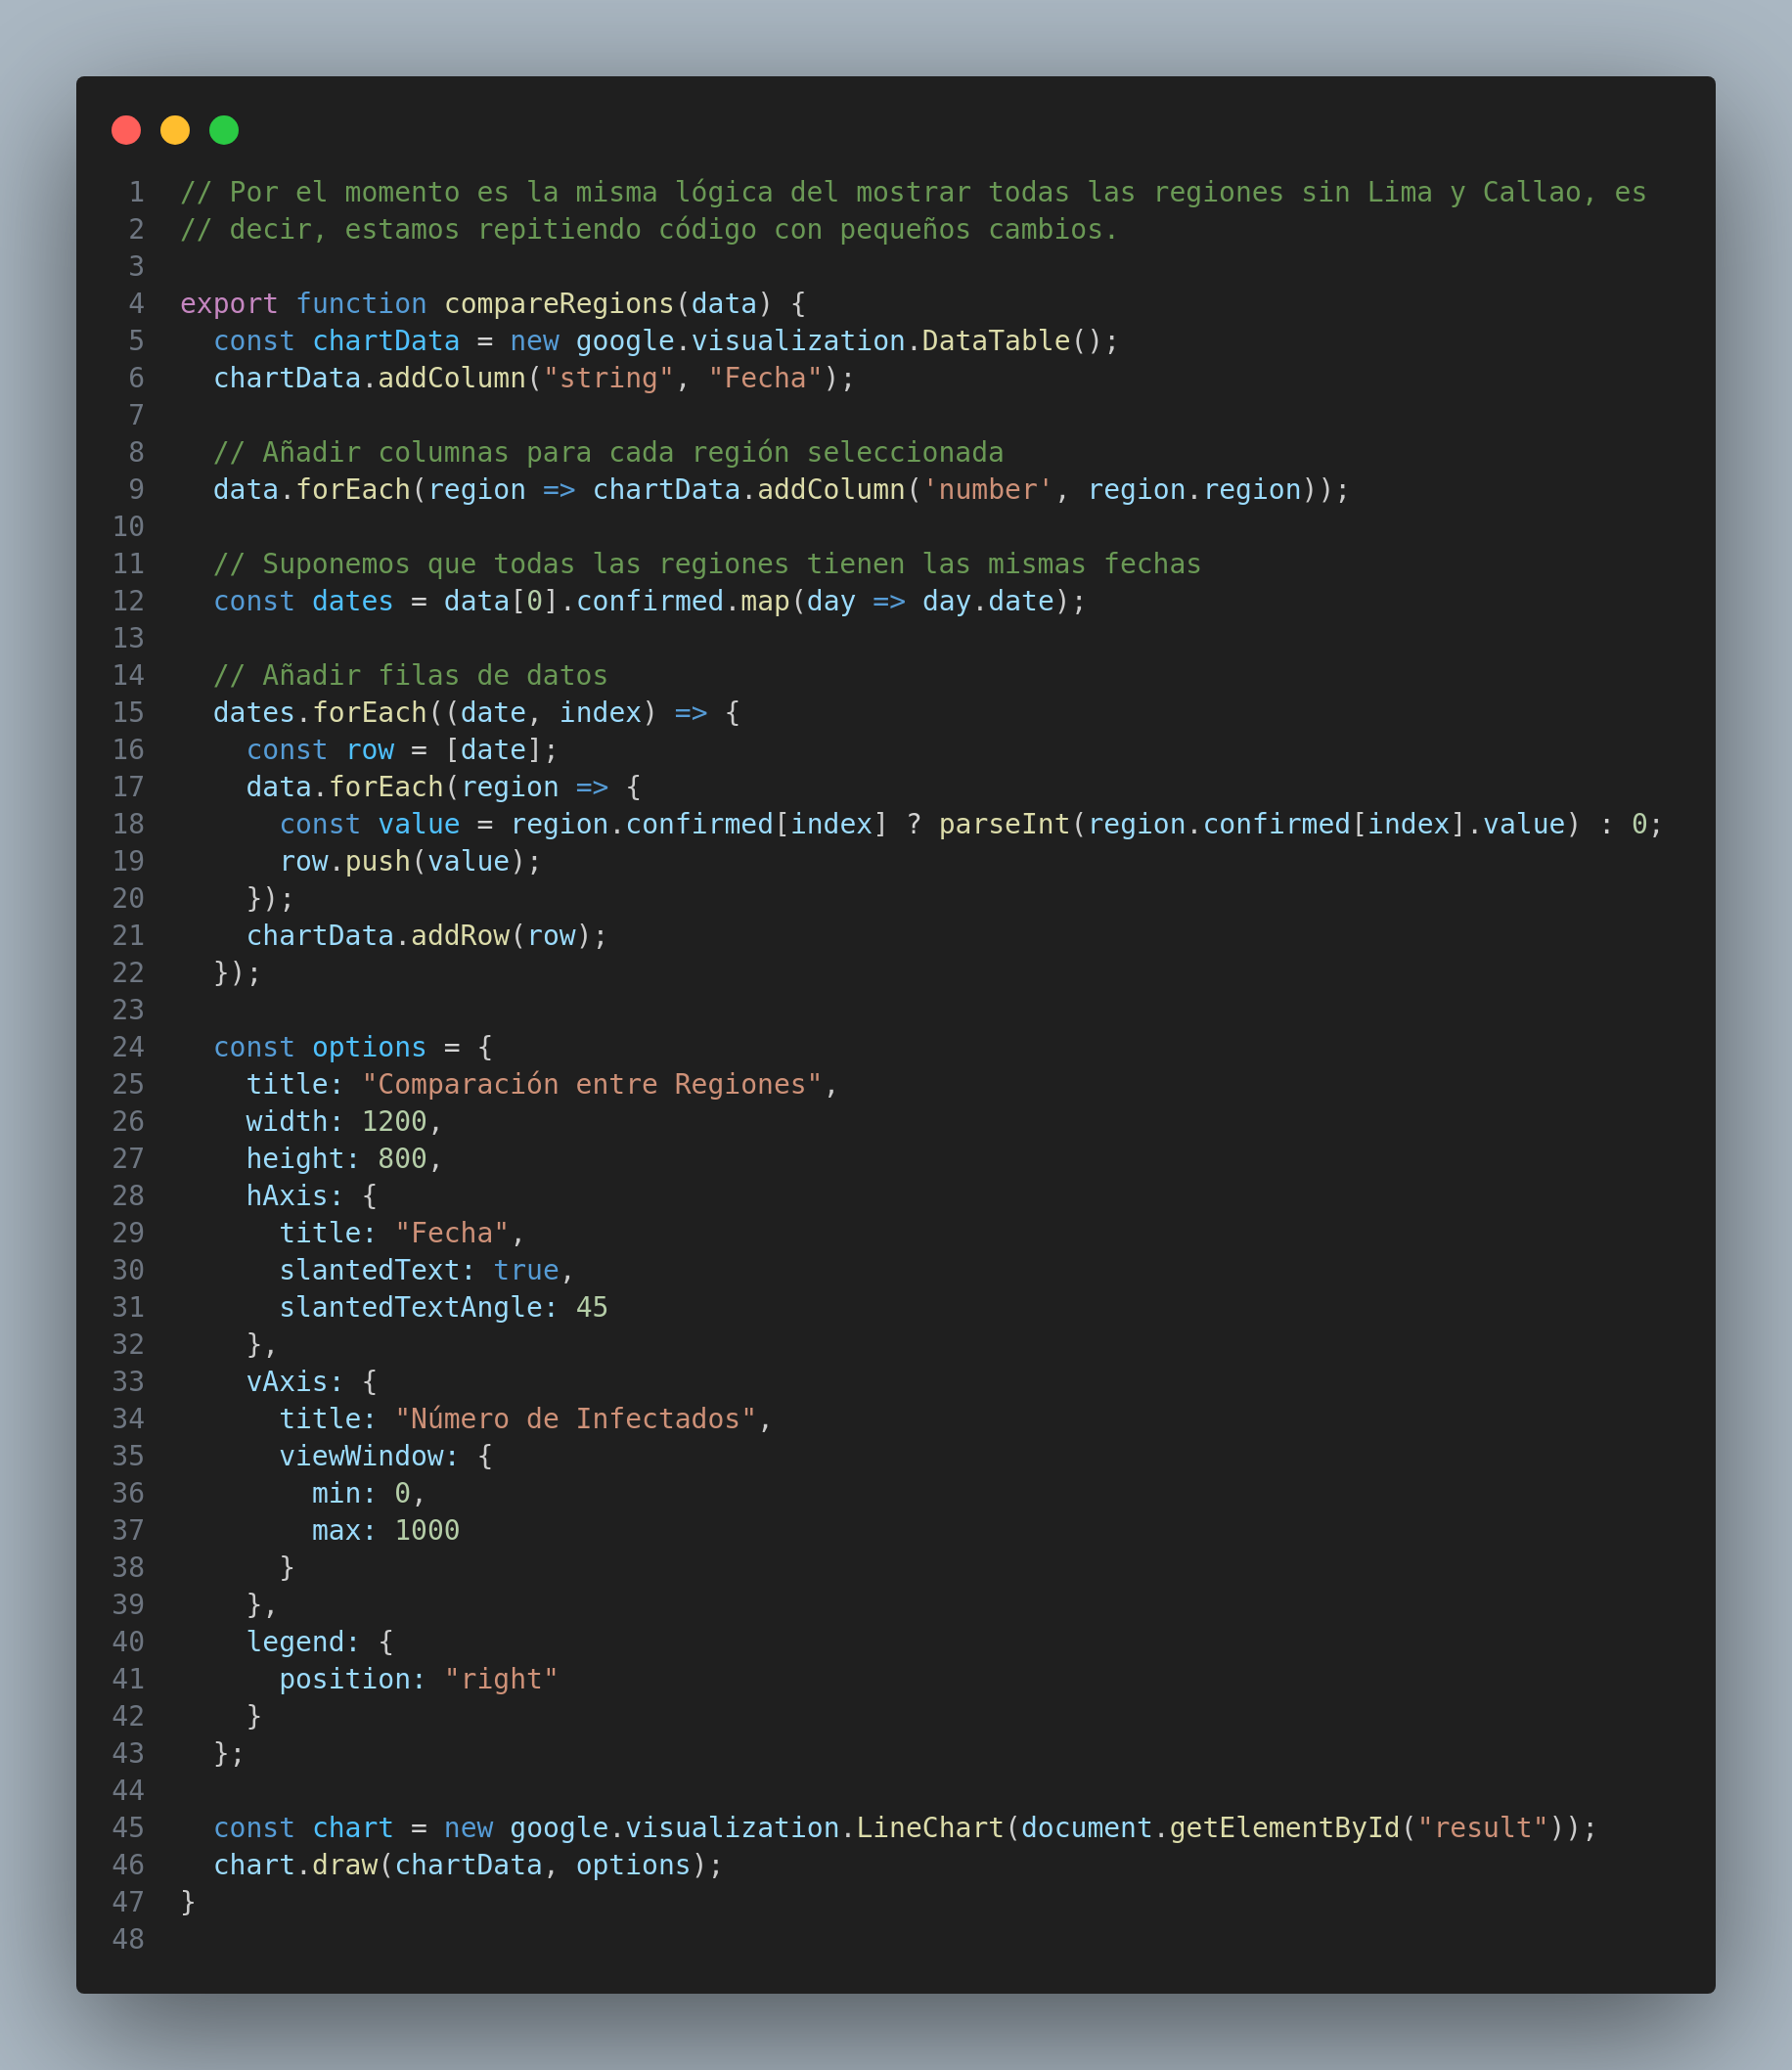
\includegraphics[width=1.0\textwidth]{img/7_js.png}
  \caption{ejercicio7.js}
\end{figure}
En el octavo ejercicio la función drawComparativeChart, genera un gráfico comparativo del crecimiento de casos de infectados en Perú, excluyendo las regiones de Lima y Callao. Filtra la información para eliminar estas dos regiones, crea una tabla de datos y prepara filas con datos de casos confirmados por fecha y región. Luego, establece opciones para el gráfico, como título y ejes, y finalmente dibuja el gráfico de líneas en un elemento HTML específico. Esta función ofrece una forma clara de comparar el avance de la enfermedad en las regiones peruanas excluyendo Lima y Callao.
\begin{figure}[H]
  \centering
  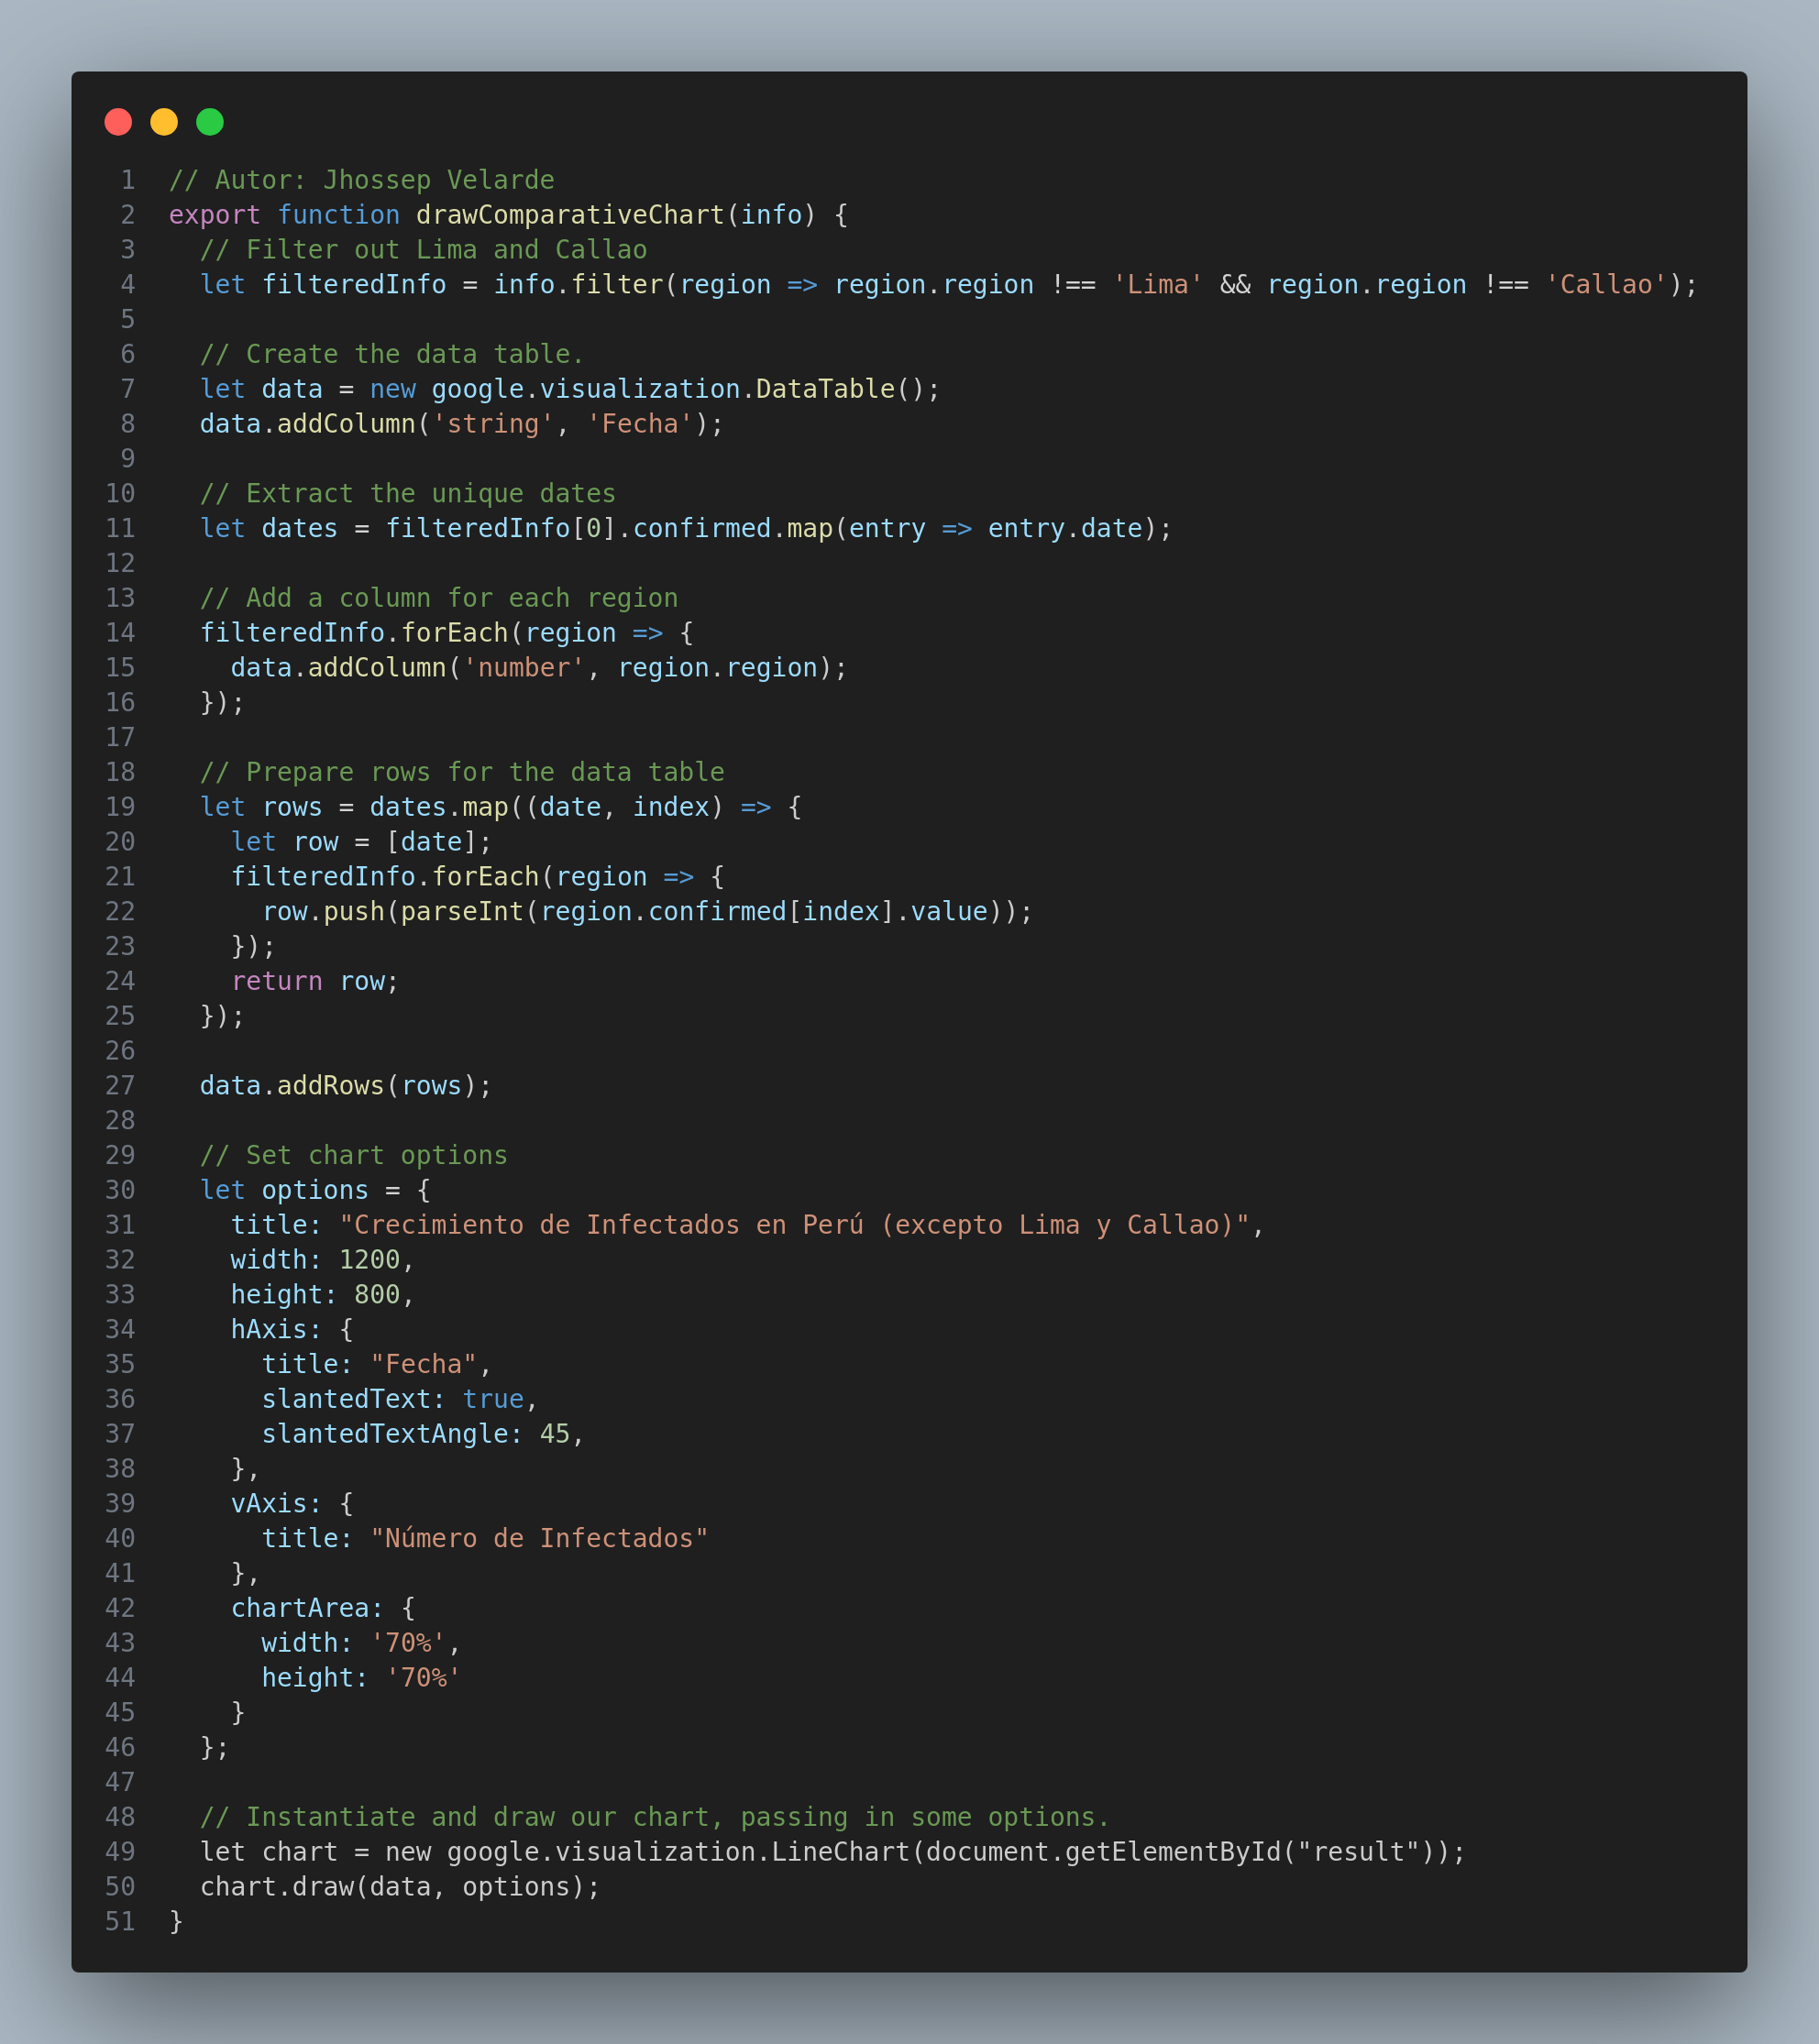
\includegraphics[width=1.0\textwidth]{img/8_js.png}
  \caption{ejercicio8.js}
\end{figure}
Tenemos un main donde se ejecutara el script importa ocho funciones desde archivos JavaScript externos, cada una diseñada para realizar una tarea específica en la visualización de datos sobre casos de infectados en regiones de Perú. Estas funciones abarcan desde la simple visualización de listas de regiones hasta la comparación detallada del crecimiento de casos confirmados en diferentes áreas geográficas. Al asociar cada función a un botón en la interfaz de usuario, el script permite una fácil interacción del usuario, lo que facilita la exploración y comprensión de los datos sobre la situación de la pandemia en Perú.
\begin{figure}[H]
  \centering
  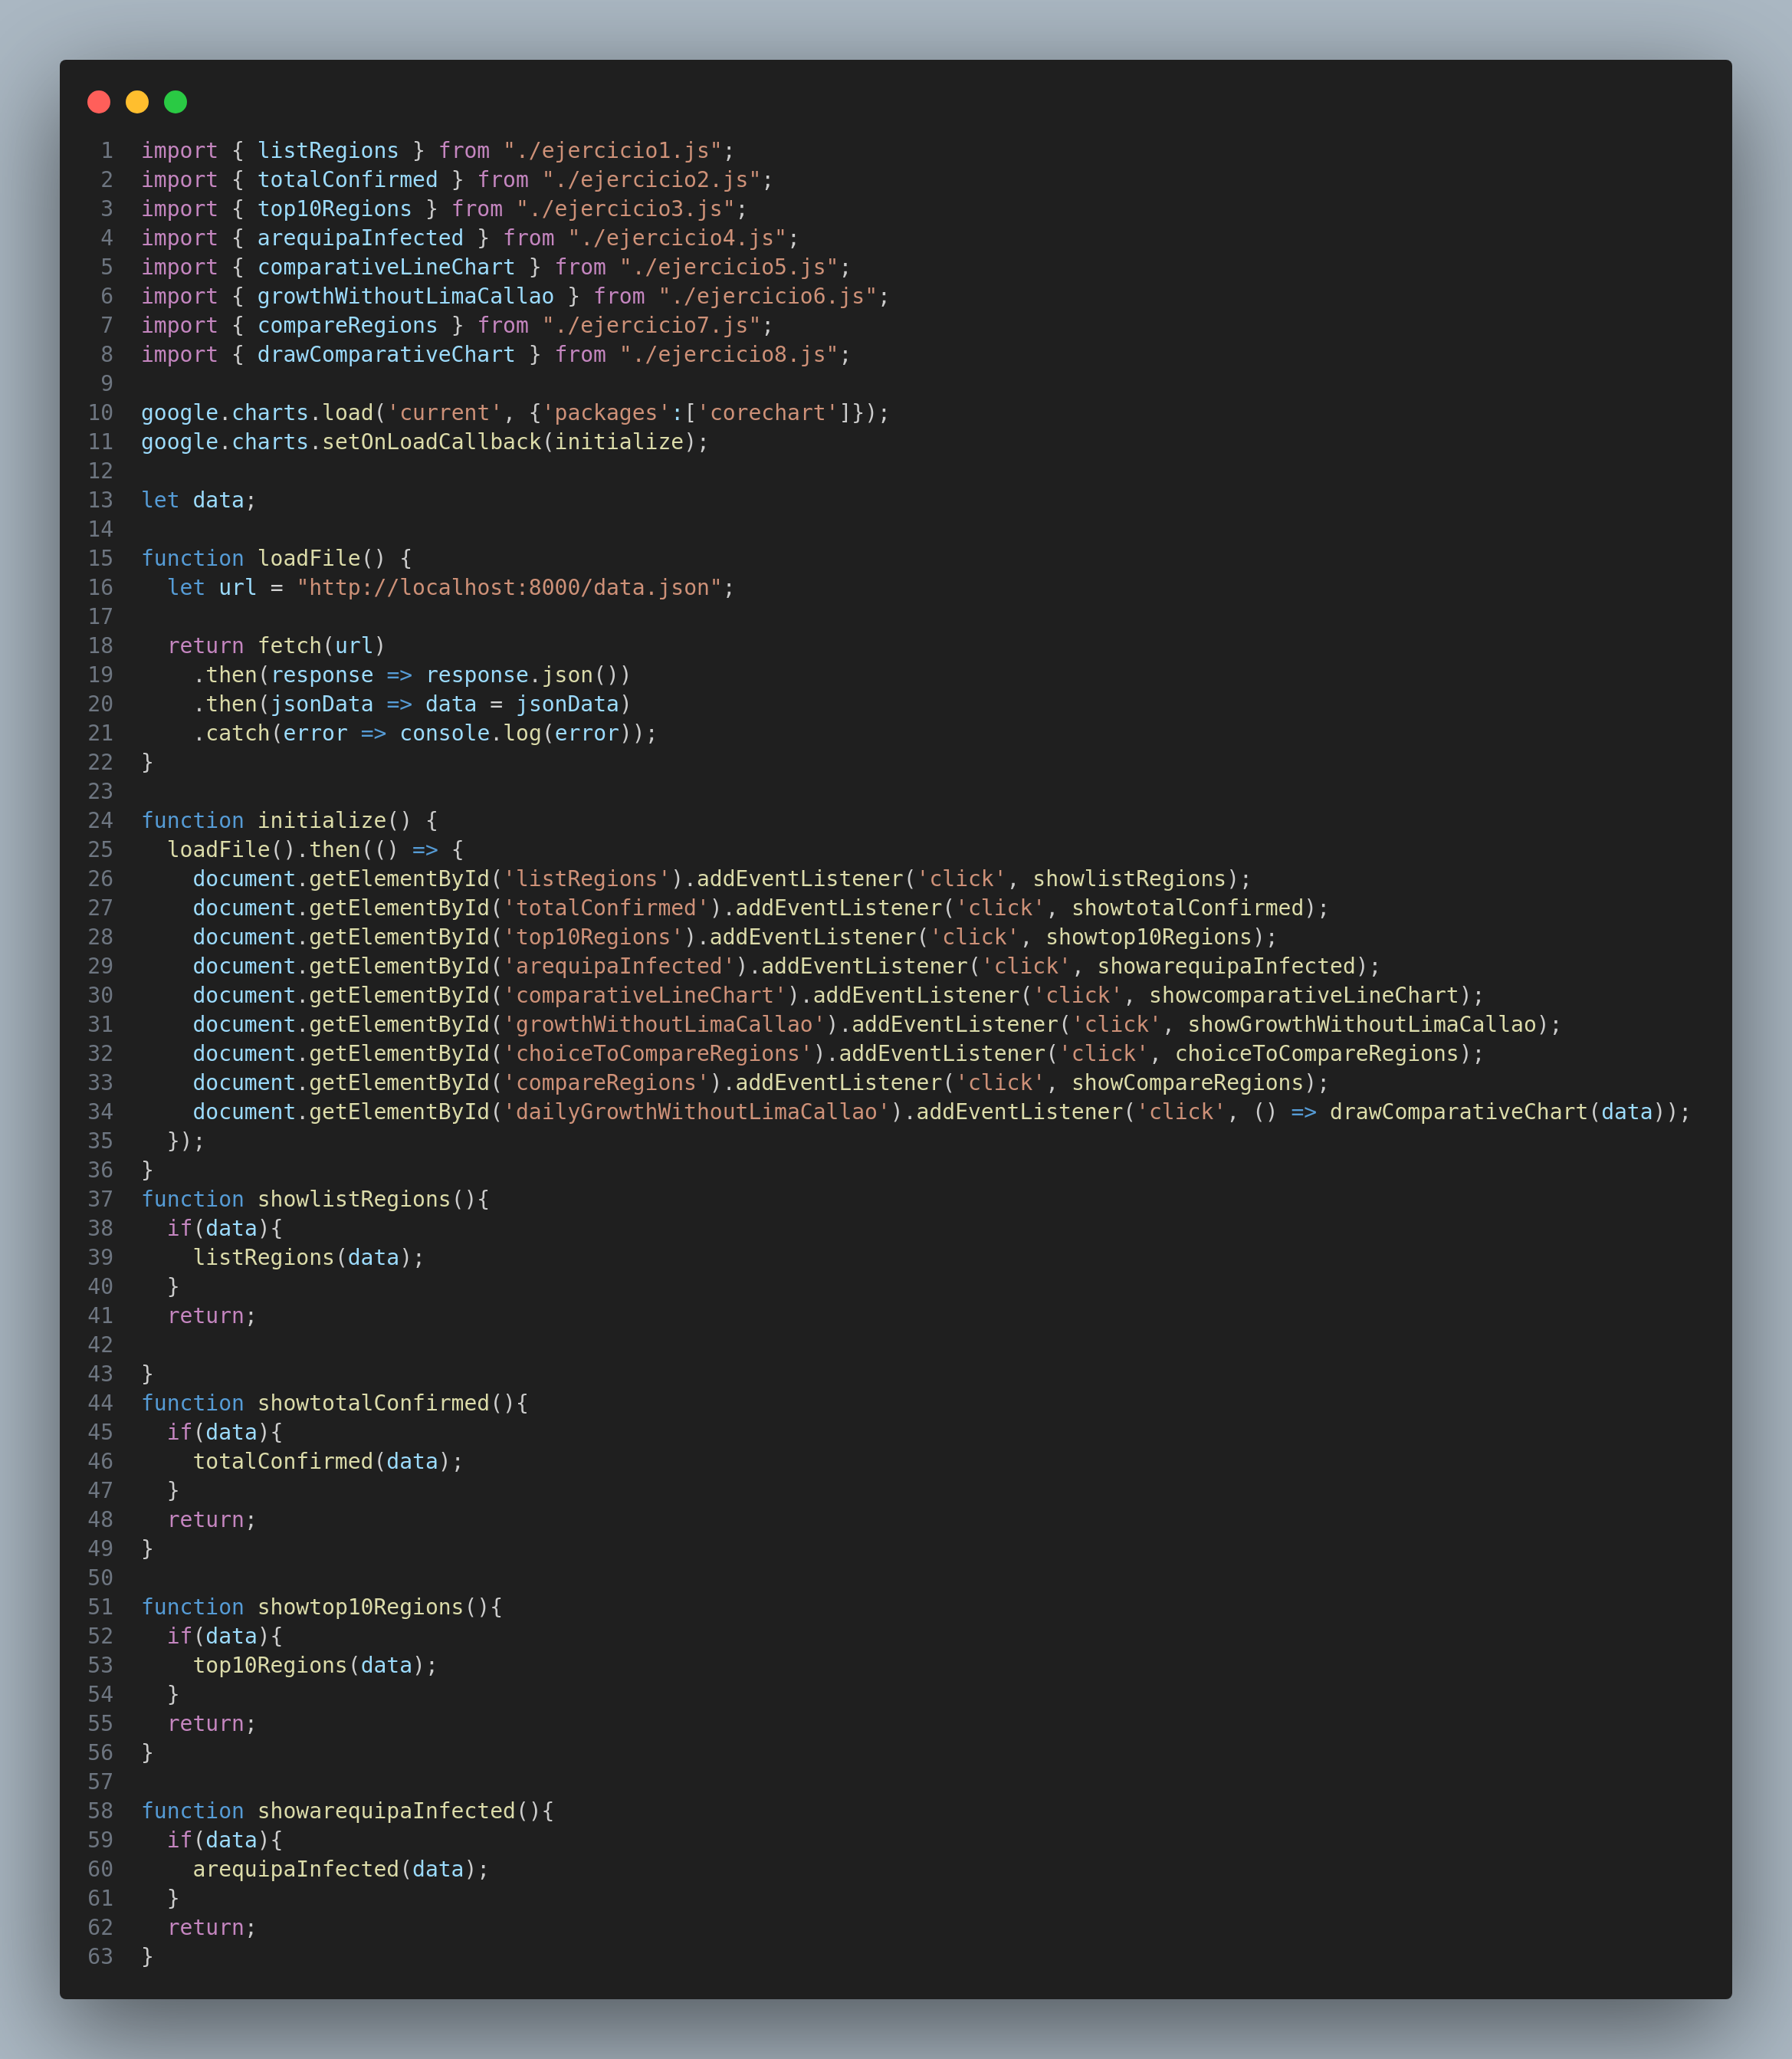
\includegraphics[width=1.0\textwidth]{img/main1_js.png}
  \caption{main.js}
\end{figure}
\begin{figure}[H]
  \centering
  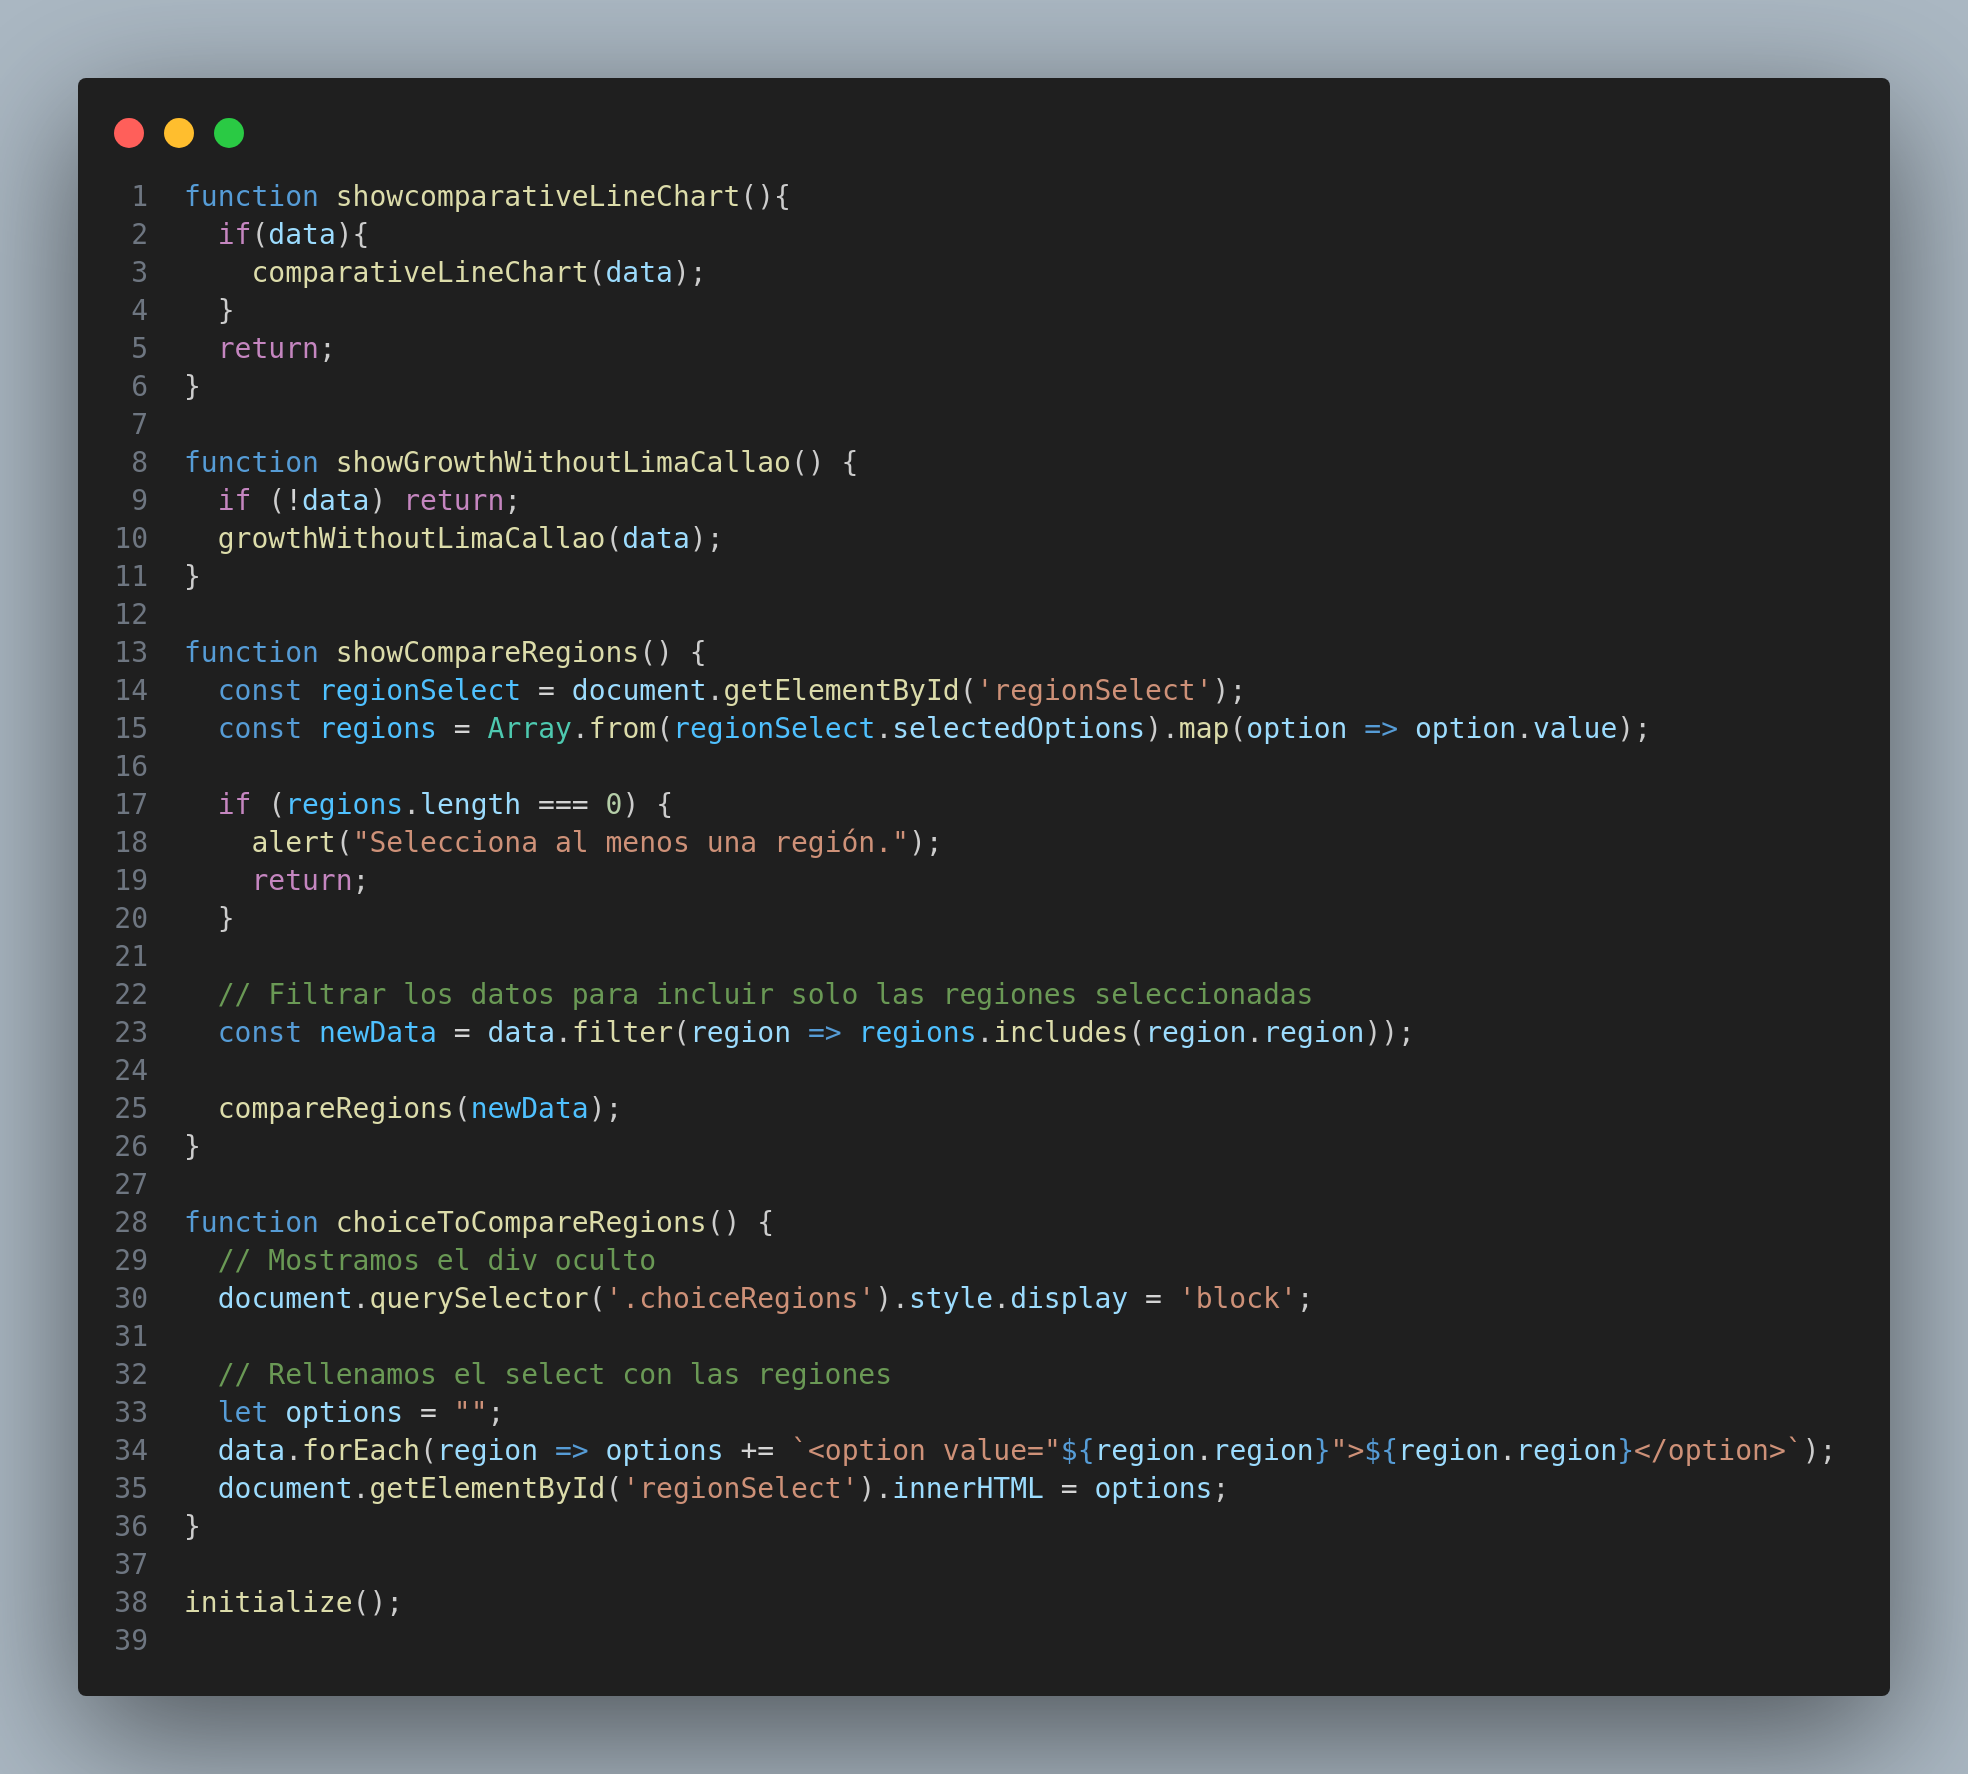
\includegraphics[width=1.0\textwidth]{img/main2_js.png}
  \caption{main.js}
\end{figure}

\section{La ejecucion de los 8 ejercicios en el index.HTML}
El primero :
\begin{figure}[H]
  \centering
  \includegraphics[width=1.0\textwidth]{img/Iniciando_Docker.png}
  \caption{Poner en funcionamiento el contenedor Docker}
\end{figure}
El segundo :
\begin{figure}[H]
  \centering
  \includegraphics[width=1.0\textwidth]{img/Iniciando_Docker.png}
  \caption{Poner en funcionamiento el contenedor Docker}
\end{figure}
El tercero :
\begin{figure}[H]
  \centering
  \includegraphics[width=1.0\textwidth]{img/Iniciando_Docker.png}
  \caption{Poner en funcionamiento el contenedor Docker}
\end{figure}
El cuarto :
\begin{figure}[H]
  \centering
  \includegraphics[width=1.0\textwidth]{img/Iniciando_Docker.png}
  \caption{Poner en funcionamiento el contenedor Docker}
\end{figure}
El quinto :
\begin{figure}[H]
  \centering
  \includegraphics[width=1.0\textwidth]{img/Iniciando_Docker.png}
  \caption{Poner en funcionamiento el contenedor Docker}
\end{figure}
El sexto :
\begin{figure}[H]
  \centering
  \includegraphics[width=1.0\textwidth]{img/Iniciando_Docker.png}
  \caption{Poner en funcionamiento el contenedor Docker}
\end{figure}
El septimo :
\begin{figure}[H]
  \centering
  \includegraphics[width=1.0\textwidth]{img/Iniciando_Docker.png}
  \caption{Poner en funcionamiento el contenedor Docker}
\end{figure}
El octavo :
\begin{figure}[H]
  \centering
  \includegraphics[width=1.0\textwidth]{img/Iniciando_Docker.png}
  \caption{Poner en funcionamiento el contenedor Docker}
\end{figure}
\end{document}
